\documentclass[sigconf]{acmart}

% Disable / remove copyright boxes
\setcopyright{none}
\settopmatter{printacmref=false}
\renewcommand\footnotetextcopyrightpermission[1]{}

% Header on each page
\acmConference[Submitted]{Submitted}{2021}{December 1st}

% Useful commands
%%%%%%%%%%%%%%%%%%%%%%%%%%%
%%% PACKAGES

\usepackage{booktabs} % For formal tables
\usepackage{algorithm}
\usepackage{algpseudocode}
\usepackage{mdframed}
\usepackage{array}
\usepackage{tabularx}
\usepackage{nicefrac}
\usepackage{balance}
\usepackage{subfigure}
\usepackage{lipsum}
\usepackage{outlines}
\usepackage{comment}
\usepackage{xcolor}
\usepackage{amsmath}
%\usepackage{amssymb}
\usepackage{amsthm}
\usepackage{url}
\usepackage{pifont}
%\usepackage[allcolors=magenta]{hyperref}
\usepackage{xspace}
\usepackage{graphics}
\usepackage{graphicx}
\usepackage{float}
\usepackage{outlines}
\usepackage{textcomp,gensymb}
\usepackage{xurl}
\usepackage{enumerate}
\usepackage{stfloats}
\usepackage{tikz}
\usepackage{enumitem}

\usepackage[normalem]{ulem} % Enables strikeout text

\mdfdefinestyle{annotex}{
    backgroundcolor=gray!10,
    innerleftmargin=0.15cm,
    innerrightmargin=0.15cm,
    leftmargin=0cm,
    rightmargin=0cm,
    font=\normalsize
}

%%%%%%%%%%%%%%%%%%%%%%%%%%%
%%% ADDITIONAL COMMANDS

% Text

% I.e.,
\newcommand{\ie}{{\it i.e.,}\xspace}

% E.g.,
\newcommand{\eg}{{\it e.g.,}\xspace}

% Math
\newcommand{\BigO}{\mathcal{O}}

% Additional table alignment
\newcolumntype{L}[1]{>{\raggedright\arraybackslash}p{#1}}
\newcolumntype{C}[1]{>{\centering\arraybackslash}p{#1}}
\newcolumntype{R}[1]{>{\raggedleft\arraybackslash}p{#1}}

%%%% Grey box

\definecolor{lightgray}{gray}{0.92}
\fboxsep2pt
\newcommand\greybox[1]{%
\vspace{6pt}%
  %\vskip 2pt%
      \par{\centering\colorbox{lightgray}{%
              \begin{minipage}{3.3in}#1\end{minipage}%
                        }%
                                    \vskip 2pt%
                                    \vspace{1pt}%
                                                }}
%%%%%%%%%%%

% Comments
\newcommand{\fix}[1]{{\textcolor{red}{[#1]}}}

\newcommand{\old}[1]{\textbf{{\textcolor{red}{#1}}}}
\newcommand{\new}[1]{\textbf{{\textcolor{blue}{#1}}}}

% Paragraph starts
\newcommand{\pstartbold}[1]{\noindent\textbf{{#1}}}
\newcommand{\pstartboldind}[1]{\vspace{0.05in}\noindent\textbf{{#1}}}
\newcommand{\pstartit}[1]{\noindent\textbf{{#1}}}
\newcommand{\pstartitind}[1]{\vspace{0.05in}\noindent\textbf{{#1}}}
\newcommand{\parab}[1]{\vspace{0.03in}\noindent{\bf #1}}

%% section/subsection spacing
\usepackage{titlesec}
\titlespacing*{\section}
{0pt}{1.2ex plus .2ex minus .2ex}{0.1ex plus .1ex}
\titlespacing*{\subsection}
{0pt}{.6ex plus .2ex minus .2ex}{0.1ex plus .05ex}
\titleformat*{\section}{\large\bfseries\scshape}

% This stops latex from leaving large spaces around figures in a column
\renewcommand{\textfraction}{0}
\renewcommand{\topfraction}{1}
\renewcommand{\bottomfraction}{1}
\setcounter{totalnumber}{10}
\setcounter{topnumber}{10}
\setcounter{bottomnumber}{10}
\setcounter{dbltopnumber}{10}
\renewcommand{\floatpagefraction}{1}
\renewcommand{\dblfloatpagefraction}{1}

% Footnote without marker
\newcommand\markerlessfootnote[1]{%
	\begingroup%
	\renewcommand\thefootnote{}\footnote{#1}%
	\addtocounter{footnote}{-1}%
	\endgroup%
}

% System name
\newcommand{\sysname}{\textsc{CodeBind}\xspace}

% ExperimenTeX
\newcommand{\experimentex}{\textsc{ExperimenTeX}\xspace}

\RequirePackage{caption, float}
\captionsetup[figure]{name={Fig.}}
\captionsetup{labelfont={bf},
    textfont={it}, labelsep=colon}

% Remove excessive space around figures
\setlength{\abovecaptionskip}{3pt plus 2pt minus 2pt}
\setlength{\belowcaptionskip}{-5pt plus 2pt minus 2pt}

%%%%%%%%%%%%%%%%%
% EXPERIMENTEX
%
% First, the five primary commands are defined.
%
% The ExperimenTeX commands are first interpreted and
% turned into runs such that afterwards the missing
% output plot files are present for the real LaTeX compilation.
% If the interpreting and plotting have not taken place,
% the LaTeX compilation will simply use placeholders.
%
% Second, two secondary commands related to checksums are defined.
%

% Package dependencies
\usepackage{color}
\usepackage{graphics}
\usepackage{graphicx}

%%%%%%%%%%%%%%%%%%%%%%%%%%%%%%%%%%%%%%%%%%%%%%%%%%%%%%%%%%%%
%
% Format:       \expclass{name-sub}{name-super}
%
% Description:  Declare the existence of class [name-sub], which inherits
%               from class [name-super]. This inheritance means it is of the same
%               experiment type, and inherits all its explines.
%
%               In the rendered document, nothing is shown.
%
\newcommand{\expclass}[2]{}

%%%%%%%%%%%%%%%%%%%%%%%%%%%%%%%%%%%%%%%%%%%%%%%%%%%%%%%%%%%%
%
% Format:       \expinstance{name-inst}{name-super}
%
% Description:  Declare the existence of instance [name-inst], which inherits
%               from class [name-super]. This inheritance means it is of the same
%               experiment type, and inherits all its explines.
%
%               In the rendered document, nothing is shown.
%
\newcommand{\expinstance}[2]{}

%%%%%%%%%%%%%%%%%%%%%%%%%%%%%%%%%%%%%%%%%%%%%%%%%%%%%%%%%%%%
%
% Format:       \expline{name}{expline}
%
% Description:  Add [expline] to the list of explines of instance/class [name].
%
%               In the rendered document, it simply shows [expline] like any other text.
%
\newcommand{\expline}[3][]{{#3}}

%%%%%%%%%%%%%%%%%%%%%%%%%%%%%%%%%%%%%%%%%%%%%%%%%%%%%%%%%%%%
%
% Format:       \expincludegraphics[ic-options]{exp-name}{output-file.ext}
%
% Description:  Add output.ext to the list of expinclude filenames of instance [name-inst].
%
%               In the rendered document, it behaves like \includegraphics.
%               If the output file does not exist (yet), a placeholder image is depicted.
%
\newcommand{\expincludegraphics}[3][]{%
\IfFileExists{../temp/plots/#2/#3}{%
\includegraphics[#1]{../temp/plots/#2/#3}%
}{%
\includegraphics[#1]{example-image-a}%
}%
}

%%%%%%%%%%%%%%%%%%%%%%%%%%%%%%%%%%%%%%%%%%%%%%%%%%%%%%%%%%%%
%
% Format:       \expincludetext{exp-name}{output-file.ext}
%
% Description:  Add output.ext to the list of expinclude filenames of instance [name-inst].
%
%               In the rendered document, it behaves like \input.
%               If the output file does not exist (yet), a placeholder red [X] is put.
%
\newcommand{\expincludetext}[2]{\IfFileExists{../temp/plots/#1/#2}{\input{../temp/plots/#1/#2}\unskip}{\textbf{\textcolor{red}{[\texttt{X}]}}}}

%%%%%%%%%%%%%%%%%%%%%%%%%%%%%%%%%%%%%%%%%%%%%%%%%%%%%%%%%%%%
%
% Format:       \expcodecksum{}
%
% Description:  Code checksum (git commit hash or archive SHA-256)
%               It is imported from file code-checksum.txt
%
\newcommand{\expcodechecksum}[0]{\IfFileExists{code-checksum.txt}{\input{code-checksum.txt}\unskip}{\textbf{\textcolor{red}{[\texttt{not found: code-checksum.txt}]}}}}


\begin{document}

% Title
\title{\sysname: tying networking papers to their experiment code}

% Shorthand authors
% \renewcommand{\shortauthors}{Kassing and Singla.}

\author{Simon Kassing}
\affiliation{
    \institution{ETH Zurich}%
    \city{}%
    \country{}%
}
\email{kassings@ethz.ch}

\author{Ankit Singla}
\affiliation{
    \institution{ETH Zurich}%
    \city{}%
    \country{}%
}
\email{asingla@ethz.ch}

\begin{abstract}
\textit{Networking research and instruction often tackle systems with a large number of configurations and possible inputs. This creates substantial complexity not only in experimentation, but also in conveying its results in papers and texts, which evolve in parallel to the experiments. First, this can cause inconsistencies between the text and its underlying experiments, requiring constant vigilance from authors. Second, the text only exposes the behavior of the studied systems across a small fraction of configurations and inputs, leaving readers with doubts about behavior in other settings.}

\textit{With \sysname, we take the first steps towards addressing these problems by: (a) bridging the gap between networking experiments and texts describing them, by having the text itself control what experiments are run; and (b) allowing readers to interact with the text and explore the behavior of the involved systems under different inputs, \textbf{without} needing any knowledge of the underlying system code. We show the utility of \sysname for the research process using three showcase sets of experiments, together with another example showing its value for teaching networking concepts.}

\end{abstract}

\begin{CCSXML}
<ccs2012>
   <concept>
       <concept_id>10011007.10011074.10011092.10011096</concept_id>
       <concept_desc>Software and its engineering~Reusability</concept_desc>
       <concept_significance>500</concept_significance>
       </concept>
   <concept>
       <concept_id>10003033.10003079.10011672</concept_id>
       <concept_desc>Networks~Network performance analysis</concept_desc>
       <concept_significance>500</concept_significance>
       </concept>
 </ccs2012>
\end{CCSXML}

\ccsdesc[500]{Software and its engineering~Reusability}
\ccsdesc[500]{Networks~Network performance analysis}

\keywords{Reproducibility, Automatic Experiment Framework}

\maketitle

\section{Introduction}

\markerlessfootnote{
    This paper is written using \sysname.\\
    \textbf{\href{https://drive.google.com/file/d/1f8gu3MpWzXM4WbpFLy7DXDcR4z3s6Ws9/view}{Demo video}} and code are available at:\\
    \url{https://github.com/snkas/codebind-paper}\\
    Code checksum: \expcodechecksum{}
}
The typical networking paper features numerous experiments and their resulting data and plots, often describing a system's behavior across a range of experiment scenarios and varied settings for parameters and configuration knobs. The resulting high complexity of writing, reviewing, and reading networking papers and texts, creates substantial challenges in ensuring their correctness, reproducibility, and relevance. 

First, the limited real-estate of a paper forces authors to pick a subset of results. Thus, only a fraction of the system's range of behaviors can be shown, with results for only some choices of the involved configuration knobs. Reviewers and readers have to rely on the authors' claims of the choices being representative. When the perspectives of reviewers and authors diverge on which configurations are most relevant, there is no easy way for reviewers to ascertain what the results would be for their preferred settings.

Second, what configurations are most relevant may change over time. For instance, the hardware costs that determine the fair comparison point between two designs could shift; or the typical operational context --- network round trip time, bandwidth, loss rate, or the relative performance of different potential bottleneck components ---  could change, making the authors' choices sub-optimal for gathering useful insights.

Third, authors manually distill experimental insights into a paper in a manner that is prone to inconsistencies arising from parallel changes made to the experiments and to the paper's text. Multiple collaborating authors, most of whom do not engage with the experimental setup, further increase the risk of disparities between what experiments are run, and what the paper's described methodology and later results state.

Lastly, it is often difficult for authors to ensure that their description of the experiments is not missing important context like the configuration parameters for the systems involved. Any missing context makes it difficult to reproduce the results. It is also non-trivial to connect text in the paper to the code for corresponding experiments within a large code repository.

Some of these problems could be addressed if readers were able to tinker with authors' code. However, for the vast majority of reviewers and readers, such deep tinkering with the authors' code is neither desirable, nor even feasible --- in fact, for the typical paper, even its senior authors do not engage with the underlying code for the experiments.

We propose to bridge the above gaps between papers and their underlying systems and experiments such that: (a) the paper's text itself determines what experiments are run; and (b) the paper's results and plots are the direct outputs of these experiments. 
Reviewers and readers (and yes, senior authors) can then modify experiment settings/parameters in the text, and see the updated results without any need to understand the authors' code. The paper's text, the experiments that are run, and their results in the paper, are all consistent by design.

Our approach, \sysname, uses a markup language in \LaTeX. The authors provide their experiment code and their paper's \LaTeX{} source. The authors use the markup in \LaTeX{} to annotate their experiments, and to create placeholders for results and plots. The same markup, minus its decorations, forms the paper text. \sysname uses the decoration to interpret the markup, and invokes the authors' experiment code to create the results. The outputs are post-processed with pipelines the authors provide to generate results and plots that replace their placeholders. 
Any changes can be easily made to the authors' markup text describing the experiments, and the paper can be regenerated with new results and plots.

This simple approach ensures that the same text that forms the body of a paper also describes the experiments that are run. Further, the results of these experiments automatically populate the text's plots and result-metrics. Making this work requires that authors use the markup appropriately and expose any parametrizable aspects of their experiment setup in this markup. However, there are healthy incentives to do so: (a) it helps authors ensure consistency and correctness; and (b) incomplete parametrization will prompt readers to question why some parametrizable aspects were not exposed.

We showcase 3 examples where readers can benefit from \sysname's interactivity: experiments on congestion control, experiments on data center network traffic, and analyzing Internet measurements. Our analysis of the NSDI 2020 program indicates that $28\%$ of papers could directly benefit from \sysname's features along the lines of our showcases, by allowing readers to tinker with experiment settings, or enabling them to explore different facets of a substantial data set. Further, nearly all papers could use \sysname to help readers delve deeper into the experimental results.

We also show \sysname's utility for teaching with an example on max-min fairness; students can interact with the example to learn the concept more deeply. Drawing on this idea, we hope to engage the community in collaboratively writing an \textit{interactive networking textbook}, making both algorithmic and systems concepts easy to explore for students.

A video demo of \sysname is \href{https://drive.google.com/file/d/1f8gu3MpWzXM4WbpFLy7DXDcR4z3s6Ws9/view}{available online}.

\section{Running example: max-min fairness}
\label{sec:example}

Consider a text intended to explain the idea of max-min fairness to students. One part of this text, explaining a consequence of max-min fairness, may read as follows:

\vspace{0.2cm}
%%%%%%%%%%%%%%%%%%%%%%%%%%%%%%%%%%%%%%%%%%%%%%%%%%%%%%%%%
\begin{mdframed}[style=annotex]

Under max-min fairness, the addition of flows to the network can \emph{increase} the throughput of some flows.

\expclass{abc}{mmfa}
To demonstrate this, we use a simple topology of three nodes with two directed edges:
\expline{abc}{the edge from A to B has a capacity of 1 unit},
and the \expline{abc}{the edge from B to C has a capacity of 1 unit}.

\expinstance{abc-one}{abc}
In the first experiment, we start the following flows: \expline{abc-one}{one from A to B} (path is A$\rightarrow$B), \expline{abc-one}{one from B to C} (path is B$\rightarrow$C), and \expline{abc-one}{one from A to C} (path is A$\rightarrow$B$\rightarrow$C).
This results in a max-min fair allocation of \expincludetext{abc-one}{flow-allocation-A-B.txt}, \expincludetext{abc-one}{flow-allocation-B-C.txt} and \expincludetext{abc-one}{flow-allocation-A-C.txt} for each.

\vspace{-0.0in}
\begin{center}
% Source file: figures/topology-example.drawio

\includegraphics[width=2.5cm]{figures/topology-example.pdf}
\end{center}
\vspace{-0.0in}

\expinstance{abc-vary}{abc}
\noindent However, say we increase the number of flows from A to B. What would happen to the flow from B to C? In the second experiment, as before, we start \expline{abc-vary}{one flow from B to C} and \expline{abc-vary}{one flow from A to C}. \expline{abc-vary}{We vary the number of flows from A to B between 1 and 4}. The addition of extra flows from A to B results in the flow from A to C being bottlenecked there, resulting in the flow from B to C being allocated more.

\begin{center}
\expincludegraphics[width=4.7cm]{abc-vary}
{num-flows-A-B-vs-flow-allocation-B-C.pdf}
\end{center}

\end{mdframed}
%%%%%%%%%%%%%%%%%%%%%%%%%%%%%%%%%%%%%%%%%%%%%%%%%%%%%%%%%
\vspace{0.2cm}

\noindent A reader can tinker with this example in several ways, including changing the capacities of the links in the topology and the number of flows between various nodes. For instance, to examine the impact of changing the capacity of the A$\rightarrow$B link to 3 units, they can edit the following line in the \LaTeX{} code:

\vspace{0.05in}
\texttt{the edge from A to B has a capacity of \old{\sout{1}} \new{3}}
\vspace{0.05in}

\noindent Similarly, to change the number of flows from A$\rightarrow$B across a wider range than above, they can edit this line:

\vspace{0.05in}
\texttt{We vary the number of flows from A to B}

\texttt{between \old{\sout{1 and 4}} \new{0 and 10}}
\vspace{0.05in}

\noindent After these small edits, the reader executes a single `refresh' command. \sysname runs the new experiments, generates plots, and inserts them to generate a new PDF document. Everything else remains as in the previous text, except the following parts that are modified, together with the new plot:

\vspace{0.2cm}
%%%%%%%%%%%%%%%%%%%%%%%%%%%%%%%%%%%%%%%%%%%%%%%%%%%%%%%%%
% NOTE: the underneath LaTeX is in a comment block, just because we do not want to simply copy-paste all the above LaTeX text to conserve space. This is done only because this is a paper *about* ExperimenTeX and we want to show how it would work.
\begin{comment}
\expclass{abc2}{mmfa}
\expline{abc2}{the edge from A to B has a capacity of 3 unit},
\expline{abc2}{the edge from B to C has a capacity of 1 unit}.
\expinstance{abc-vary2}{abc2}
\expline{abc-vary2}{one flow from B to C}
\expline{abc-vary2}{one flow from A to C}
\expline{abc-vary2}{We vary the number of flows from A to B between 0 and 10}
\end{comment}

\begin{mdframed}[style=annotex]
\ldots the edge from A to B has a capacity of \textbf{3} \ldots\\
\ldots This results in a max-min fair allocation of \textbf{2.5, 0.5 and 0.5} for each flow respectively. \ldots\\
\ldots We vary the number of flows from A to B between \textbf{0 and 10}. \ldots
\begin{center}
\expincludegraphics[width=4.7cm]{abc-vary2}
{num-flows-A-B-vs-flow-allocation-B-C.pdf}
\end{center}
\end{mdframed}
%%%%%%%%%%%%%%%%%%%%%%%%%%%%%%%%%%%%%%%%%%%%%%%%%%%%%%%%%
\vspace{0.2cm}

\vspace{0.05in}
\noindent \textbf{We welcome readers to themselves make modifications in the \LaTeX{} code for the full text block at the start of this section to see how the text and results change in place.} This example illustrates the simplicity of a reader interacting with a \sysname-enabled paper. It is up to the authors how much of an experiment is exposed for interaction. Parts of the experiment can be left fixed, such as the topology in the above example. We will next use the same example to detail \sysname's design and the authors' perspective.

\section{\sysname design}
\label{sec:system-design}

\sysname is designed to impose minimal burden on authors. The benefit of automatic consistency between the experiments and the text should provide more than sufficient incentive for the minor effort required to use \sysname.

%%%%%%%%%%%%%%%%%%%%%%%%%%%%%%%%%%%%%%%%%%%%%%%%%%%%%%
%%%%%%%%%%%%%%%%%%%%%%%%%%%%%%%%%%%%%%%%%%%%%%%%%%%%%%
%%%%%%%%%%%%%%%%%%%%%%%%%%%%%%%%%%%%%%%%%%%%%%%%%%%%%%
%%%%%%%%%%%%%%%%%%%%%%%%%%%%%%%%%%%%%%%%%%%%%%%%%%%%%%
%%%%%%%%%%%%%%%%%%%%%%%%%%%%%%%%%%%%%%%%%%%%%%%%%%%%%%

\subsection{Overview}
\label{sec:workflow}

At a high level, \sysname augments \LaTeX{} with a markup language to: (a) capture inputs to the experiments; and (b) create placeholders for text and plots showing results. When the marked-up \LaTeX{} source is compiled, \sysname parses the inputs and invokes the authors' experiment code. For creating the final PDF, the generated results are used to replace placeholders in the text.
End-to-end, the following steps, as illustrated in Fig.~\ref{fig:architecture}, create a \sysname-enabled paper:


\begin{itemize}[leftmargin=12pt,itemsep=2pt,topsep=2pt]
    \item The authors use a lightweight markup language to annotate inputs, parameters, configurations, etc. in their \LaTeX{} source. They also annotate placeholders for text about results, as well as result plots.
    \item \sysname interprets the markup throughout the paper in a single pass, and creates input files for the authors' experiment framework(s). Each experiment is executed with its specified inputs to generate the outputs.
    \item \sysname invokes the authors' post-processing routine(s) to generate any plots and result metric values with the labels matching the corresponding placeholders.
    \item The last step is a traditional \LaTeX{} compilation, not specific to \sysname, to create the document.
\end{itemize}

\noindent A key design choice is to not overly restrict how experiments are specified, \eg with a limited domain-specific language. Instead, given the diversity of experimental methods and frameworks, \sysname relies on general purpose hooks to invoke the authors' experiment framework(s) with appropriate input and output files. The authors themselves decide what constitutes an experiment, and how it can be modified, parameterized, analyzed, and presented. The authors use the markup to express these decisions, and provide means to invoke their experiment framework(s) with the input files \sysname creates from parsing the markup. The experiment framework can be \emph{anything} that: (a) accepts input files and outputs result / log files; and (b) can be executed by others without depending on custom hardware, bespoke testbeds, etc.

Today's typical workflow involves experiment run scripts in authors' code, which the authors execute, and manually extract the resulting data and plots from, to add to their paper's text. In contrast, \sysname makes the paper's text itself the collection of ``run scripts'', using them to control the experiments, and to automatically ingest the resulting outputs.

% Architecture overview
\begin{figure}
 \begin{center}
  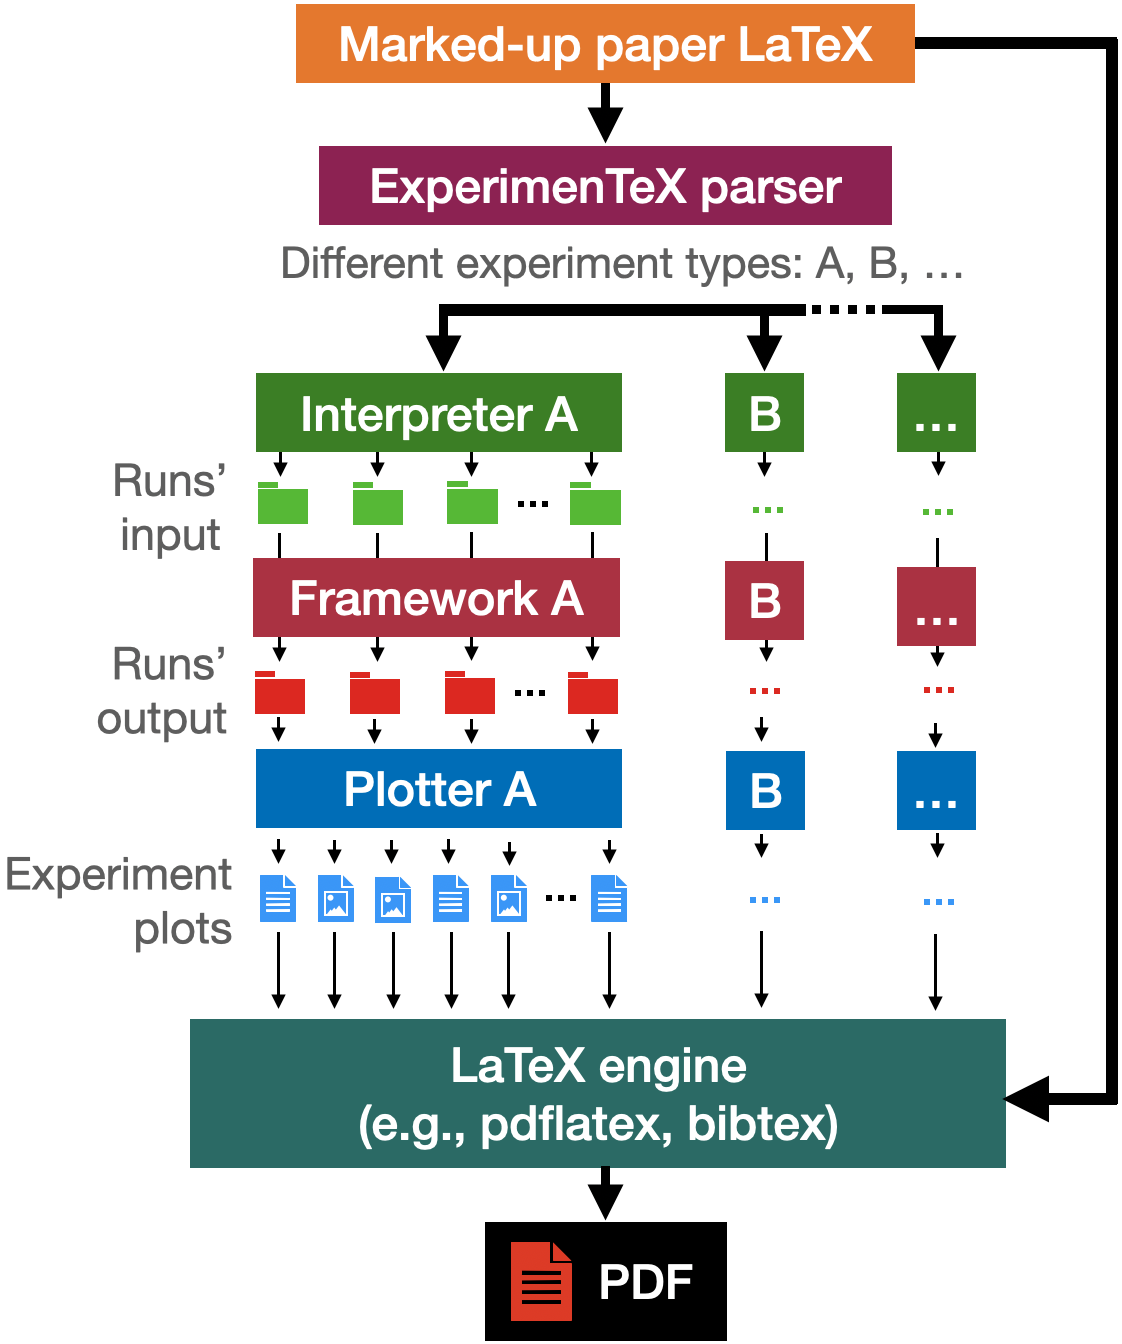
\includegraphics[width=0.47\textwidth]{figures/architecture.png}
  \caption{\sysname overview: authors use simple markup in \LaTeX{}, which our parser parses. Authors' code itself must translate the parsed representations to create inputs for the authors' experiment framework(s), and to identify the result text and plots needed. The experiments are invoked on the inputs, and the authors' post-processing and plotting pipelines are used to generate the result text and plots. A standard \LaTeX{} compile uses these resources to create the PDF.}
  \vspace{-5pt}
  \label{fig:architecture}
  \vspace{0pt}
 \end{center}
\end{figure}

%%%%%%%%%%%%%%%%%%%%%%%%%%%%%%%%%%%%%%%%%%%%%%%%%%%%%%
%%%%%%%%%%%%%%%%%%%%%%%%%%%%%%%%%%%%%%%%%%%%%%%%%%%%%%
%%%%%%%%%%%%%%%%%%%%%%%%%%%%%%%%%%%%%%%%%%%%%%%%%%%%%%
%%%%%%%%%%%%%%%%%%%%%%%%%%%%%%%%%%%%%%%%%%%%%%%%%%%%%%
%%%%%%%%%%%%%%%%%%%%%%%%%%%%%%%%%%%%%%%%%%%%%%%%%%%%%%

\subsection{\experimentex markup}
\label{sec:experimenttex}

\sysname's markup language, \experimentex, provides two types of primitives corresponding to its two main tasks:

\parab{explines:} An expline, a portmanteau of "experiment" and "line", is a line of text that defines (part of) a particular experiment's setup, including its parameters and configurations. In the max-min fairness example (\S\ref{sec:example}), ``\texttt{the edge from 1 to 2 has a capacity of 1 unit}'' is an expline.

\parab{expincludes:} An expinclude, a portmanteau of "experiment" and "included file", is a placeholder for result text and result plots. In the max-min fairness example, the flows' computed allocation in the text, as well as the plot, used expincludes.

\vspace{0.1in}
\noindent\experimentex wraps explines and expincludes in an object-oriented paradigm. An experiment class, \textbf{expclass}, defines a type of experiment, while an experiment instance, \textbf{expinstance}, completes the specification of a particular experiment by instantiating an experiment class.

Both expclasses and expinstances can have explines declared to belong to them. The difference is that an expclass is, by definition, incomplete: its explines do not fully define all aspects of the experiment's setup, whereas for an expinstance, they must fully cover the experiment's setup. For every type of experiment, authors define an empty root expclass, which does not have any explines, and can only be inherited from. Authors can declare multiple subclasses inherited from the same expclass, to prevent the repetition of text describing similar experiments. Finally, only expinstances, by virtue of completing the specification for an experiment, can have expincludes to host experiment results.

In sum, \experimentex is a collection of the following $5$ minimally obtrusive \LaTeX{} commands that the authors of a \sysname-enabled paper must use:

\begin{itemize}[leftmargin=12pt,itemsep=2pt,topsep=2pt]
    \item \texttt{\textbackslash expclass\{name-sub\}\{name-super\}}\vspace{0.05cm}\\
          Declare class \texttt{name-sub}, which inherits from class \texttt{name-super}. This inheritance means it is of the same experiment type, and inherits all its explines.
          \vspace{0.1cm}
    \item \texttt{\textbackslash expinstance\{name-inst\}\{name-super\}}\vspace{0.05cm}\\
          Declare experiment instance \texttt{name-inst}, which inherits from expclass \texttt{name-super}. This inheritance means it is of the same experiment type, and inherits all its explines.
          \vspace{0.1cm}
    \item \texttt{\textbackslash expline[identifier (opt)]\{name\}\{\textbf{expline}\}}\vspace{0.05cm}\\
          Add \texttt{expline} to the list of explines of expinstance or expclass. The \texttt{identifier} option can be used to inform the interpreter what the expline describes, \eg \\ \texttt{\textbackslash expline[link-data-rate]\{example\}\{10~Mbit/s\}}.\\ This is useful for specifying standalone parameters.
          \vspace{0.1cm}
    \item \texttt{\textbackslash expincludetext\{name-inst\}\{\textbf{out.ext}\}}\vspace{0.05cm}\\
          Add out.ext to the expincludes of instance \texttt{name-inst}.
          \vspace{0.1cm}
    \item \texttt{\textbackslash expincludegraphics[...]\{name-inst\}\{\textbf{out.ext}\}}\vspace{0.05cm}\\
          Add out.ext to the expincludes of instance \texttt{name-inst}.\vspace{0.1cm}
\end{itemize}

\begin{figure*}
    \centering
    % Source file: figures/markup-example.key
    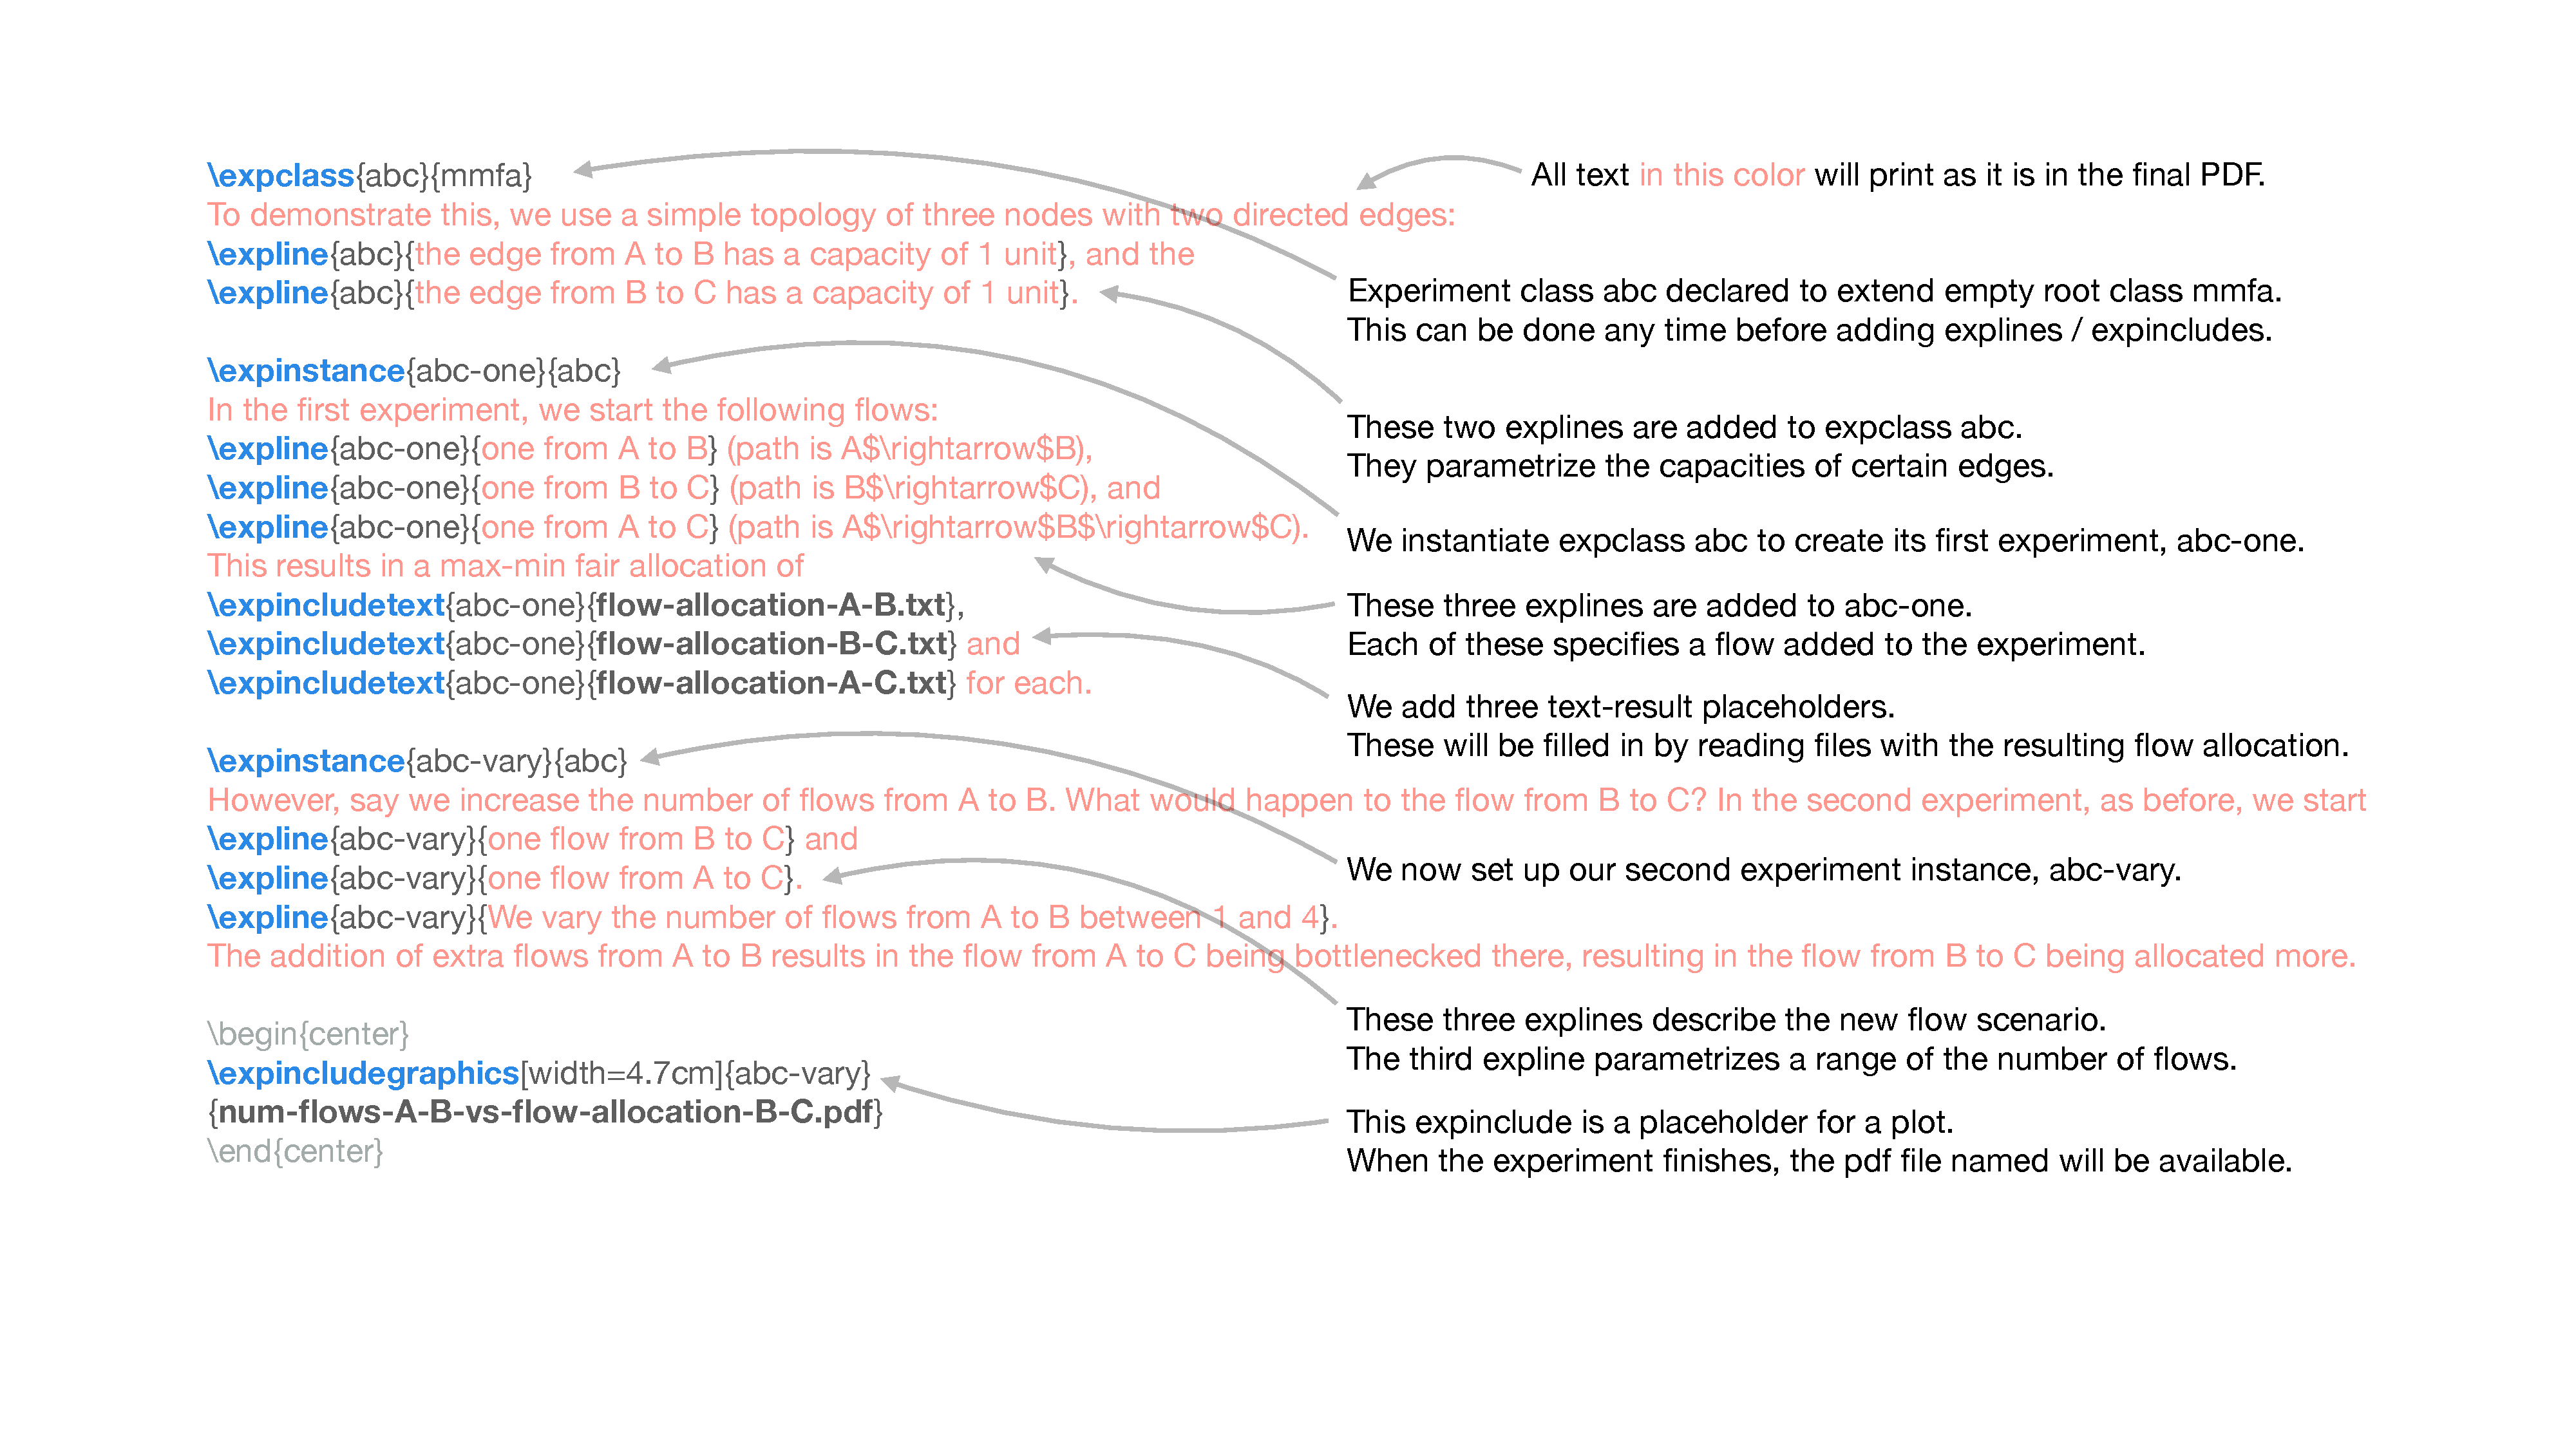
\includegraphics[width=\textwidth]{figures/markup-example.pdf}
    \caption{\LaTeX{} source for the max-min fairness example. There are two experiment instances \texttt{abc-one} and \texttt{abc-vary}, both of which inherit from class \texttt{abc}. The flow scenarios are described for each using \texttt{explines}. For the first experiment, three text results, one value for each of the three flow allocations, will be read from the files specified after the experiment runs. For the second one, the plot in the file specified using \texttt{expincludegraphics} will be inserted.}
    \label{fig:example-latex}
    \vspace{-6pt}
\end{figure*}

\noindent All of the above markup is used internally by our \experimentex parser (and subsequently, author-defined interpretations of it), but only the \textbf{bold} parts have direct, visible impact on the final PDF document compiled by \LaTeX{}. The explines are printed as is --- this is key to ensuring consistency between what is written and what is run in the experiments. The two types of expincludes behave like the \texttt{\textbackslash{}input} and \texttt{\textbackslash{}includegraphics} \LaTeX{} commands, and are used to add result text and result plots respectively.

Fig.~\ref{fig:example-latex} shows the \LaTeX{} code for the max-min fairness example from \S\ref{sec:example}. Some superfluous parts, like the opening preamble text and the topology graphic, are excluded for brevity.

By default, all \experimentex commands are ``safe'' in that they do not cause warnings or errors if the \LaTeX{} source is compiled without running the experiments via \sysname. In this case, the placeholders for experiment results simply show default text and figure placeholders --- Appendix~\ref{sec:compile-like-normal} shows what this looks like for the max-min fairness text. The grammatical validity, \eg inheritance and naming, is only appraised when the \experimentex parser runs (\S\ref{sec:parser}). Whether the explines translate to valid runs is only determined once the interpreter runs over the parser's output (\S\ref{sec:interpreter}). The validity of the output results is only determined once the plotter has run over the parser's output representation, combined with the runs' output log files (\S\ref{sec:plotter}).

%%%%%%%%%%%%%%%%%%%%%%%%%%%%%%%%%%%%%%%%%%%%%%%%%%%%%%
%%%%%%%%%%%%%%%%%%%%%%%%%%%%%%%%%%%%%%%%%%%%%%%%%%%%%%
%%%%%%%%%%%%%%%%%%%%%%%%%%%%%%%%%%%%%%%%%%%%%%%%%%%%%%
%%%%%%%%%%%%%%%%%%%%%%%%%%%%%%%%%%%%%%%%%%%%%%%%%%%%%%
%%%%%%%%%%%%%%%%%%%%%%%%%%%%%%%%%%%%%%%%%%%%%%%%%%%%%%

\subsection{Parsing \experimentex}
\label{sec:parser}

The parser uses the TexSoup package~\cite{texsoup} for the initial TeX parsing, but only targets the found \experimentex commands in the \LaTeX{} source. The authors supply the parser with a list of root experiment class names. For each root class, the parser outputs a tree, whose directed edges represent the inheritance between experiment instances and classes, which are its nodes. Every node has a list of explines. Only the leaves, \ie experiment instances, additionally have a list of expincludes. The interpreter uses the parsed tree to create and performs runs, and the plotter uses it to (after the runs) know which outputs to generate. The parser guarantees that the tree satisfies various constraints, \eg names must be declared first and must be unique; after extending a class, it cannot have more explines declared; and instances cannot be extended from.

In our running example, there is only one root class, \texttt{mmfa}, so only one tree is output by the parser, shown in Fig.~\ref{fig:parsed-tree}.

The parser creates the tree, but does not check whether the explines are valid, which is the interpreter's task (see \S\ref{sec:interpreter}), nor does it check whether the expinclude filenames are valid, which is the plotter's task (see \S\ref{sec:plotter}). As such, the parser is the same for all \sysname papers, and does not need to be edited by the authors.

\begin{figure}
    \centering
    % Source file: figures/parsed-tree.key
    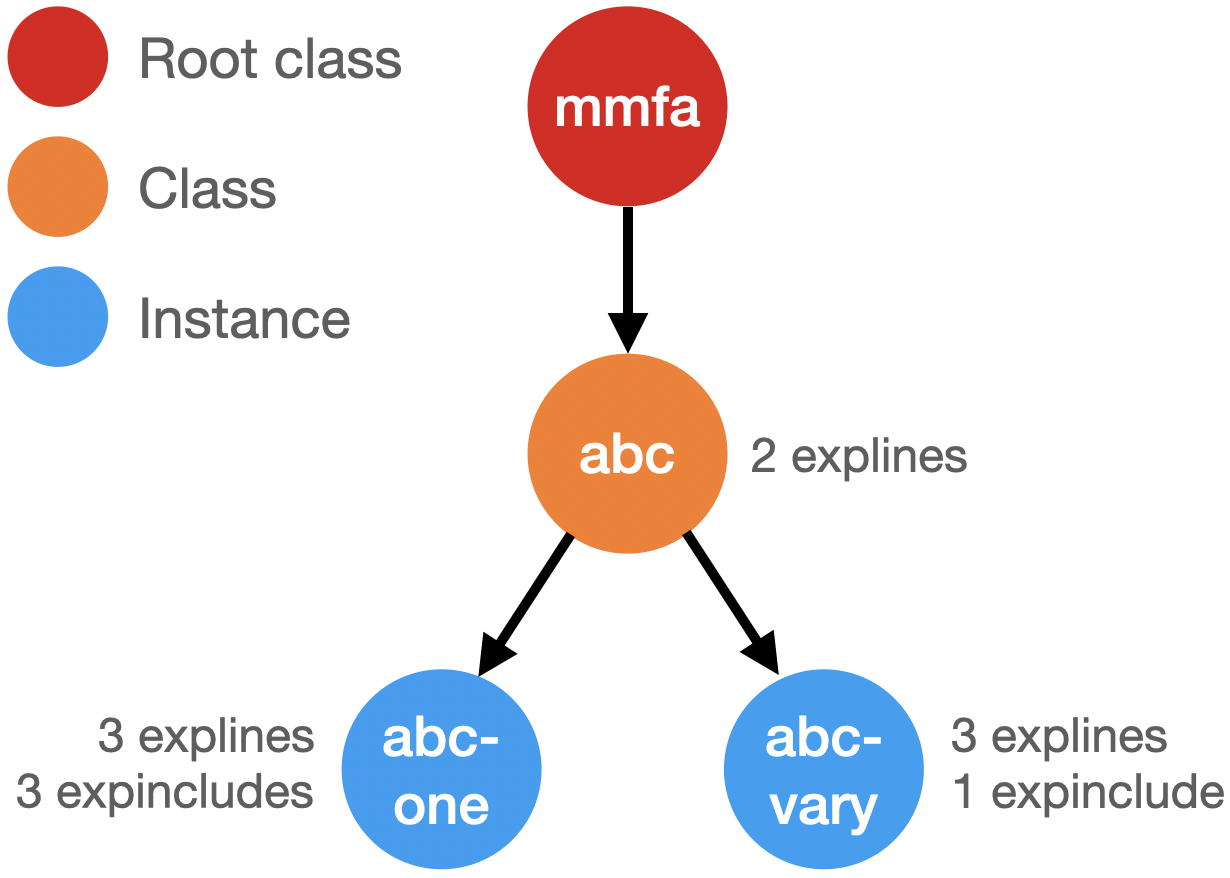
\includegraphics[width=0.3\textwidth]{figures/parsed-tree.png}
    \caption{Parsed tree for the max-min fairness example of \S\ref{sec:example}.}
    \label{fig:parsed-tree}
    \vspace{-14pt}
\end{figure}

%%%%%%%%%%%%%%%%%%%%%%%%%%%%%%%%%%%%%%%%%%%%%%%%%%%%%%
%%%%%%%%%%%%%%%%%%%%%%%%%%%%%%%%%%%%%%%%%%%%%%%%%%%%%%
%%%%%%%%%%%%%%%%%%%%%%%%%%%%%%%%%%%%%%%%%%%%%%%%%%%%%%
%%%%%%%%%%%%%%%%%%%%%%%%%%%%%%%%%%%%%%%%%%%%%%%%%%%%%%
%%%%%%%%%%%%%%%%%%%%%%%%%%%%%%%%%%%%%%%%%%%%%%%%%%%%%%

\subsection{Interpreter: invoking experiments}
\label{sec:interpreter}

For each root experiment class, $r$, the authors write an interpreter. The interpreter takes $r$'s parsed tree, and translates it into experiment runs that can be executed by the authors' chosen frameworks. Writing an interpreter entails four tasks.

\parab{Task 1: define the root data structure}\\
The interpreter defines an empty root data structure, which contains the parameters that can be set by explines.

In our running example, we want to experiment with a (fixed) three node topology with two directed links (A$\rightarrow$B, B$\rightarrow$C). There are two parametrizable aspects: the link capacities and the flow scenario. We thus define root class \texttt{mmfa} with the following data structure:
\vspace{-0in}
\begin{verbatim}
DATA STRUCTURE mmfa {
  cap_A_B: float
  cap_B_C: float
  num_flows_A_B: integer (or list[integer])
  num_flows_B_C: integer (or list[integer])
  num_flows_A_C: integer (or list[integer])
}
\end{verbatim}
\vspace{-0in}
\noindent To allow multiple runs across a range of values for a parameter, we use lists in the data structures. In the above example, the number of flows between each pair of nodes can be varied. If each of the three flow counts uses such a range instead of one value, we end up with a Cartesian product of runs.

\parab{Task 2: interpret explines into data structures}\\
The interpreter goes through the parsed tree starting from the root, and interprets the explines defined for each node to fill in the data structure. Every child of a node receives a copy of the data structure of its parent, thus inheriting all its explines. Each leaf must end up with a fully filled-in root data structure. Only leaves, \ie experiment instances, will be converted into one or more run directories for a certain framework.

What constitutes a valid expline, its \textit{template}, must be intuitive and its effect on the underlying data structure predictable. However, the explines are sentences which will literally be displayed in the final paper: we do not want to restrict authors to being only able to form rigid flow-breaking sentences because they must match a certain format. The best of both worlds can be achieved by combining regular expression (regex) matching (deterministic, but rigid) with an iterative writing approach (\S\ref{sec:writing-strategy}). Every iteration after the authors have edited the text, they add, extend and/or update the regular expression and the parsing of their grouped values. Typically, few changes are required in the interpreter apart from the addition, removal and reordering of filler words in the regex pattern.

The explines are processed sequentially in deterministic reading order from the start to the end of the paper's LaTeX. The interpreter must evaluate explines and update the data structure accordingly. The interpreter throws an error if the expline does not match a template, if the values are incorrect, or if the expline is invalid given the current state of the data structure (\eg due to conflict with a previous expline).

For our running example, we define the following templates to be valid for our interpreter:
\vspace{-0in}
\begin{verbatim}
(1) The edge from {} to {} has a capacity of {}
(2) We vary the number of flows 
    from {} to {} between {} and {}
(3) One from {} to {}
(4) One flow from {} to {}
\end{verbatim}
\vspace{-0in}
\noindent The interpreter first performs regular expression (regex) matching to identify the groups. In the regex-matching, we make sure that it is resistant whether the first letter capitalized or if there is an ending dot, and which type of white space exists between the words. The regex groups are values which are subsequently verified. It must enforce constraints such that the data structure is modified correctly: it throws an error, for example, if the values contain invalid node identifiers, non-existent links, or negative capacities. An expline must also be consistent with the effect of explines which came before, \eg setting the capacity of a link twice is not permitted. 

For greater writing flexibility, authors can iteratively augment the set of valid templates, for instance, in the above example, it may be useful to add a template to specify the capacity of all links at once.

For our example, the interpreter receives the parsed tree of Fig.~\ref{fig:parsed-tree}. It first interprets the 2 explines for class \texttt{abc} into its data structure. Afterward, the interpreter creates two copies of the data structure for the two child classes \texttt{abc-one} and \texttt{abc-vary}, and then processes the additional explines for each of them. This results in two completely filled data structures, one for each experiment instance:
\vspace{0in}
\begin{verbatim}abc-one {
  cap_A_B: 1,
  cap_B_C: 1,
  num_flows_A_B: 1,
  num_flows_B_C: 1,
  num_flows_A_C: 1
}
abc-vary { 
  cap_A_B: 1,
  cap_B_C: 1,
  num_flows_A_B: [1, 2, 3, 4],
  num_flows_B_C: 1,
  num_flows_A_C: 1
}\end{verbatim}
\vspace{-0in}
\noindent\textbf{Task 3: translate data structures into run directories}\\
The interpreter prepares for invoking the authors' run framework(s) by creating a directory for each individual run. If an experiment instance's data structure only has attributes which are single-valued, it will directly map to a single run directory. If it has attributes which are multi-valued, it leads to a Cartesian product of single-valued data structures, and an equal number of run directories. A run directory is thus self-contained from the perspective of the run framework, providing both the inputs and a location for the outputs. The directory translation has the following components:

\begin{itemize}[leftmargin=12pt,itemsep=2pt,topsep=2pt]

    \item \textbf{Naming and look-up.} We name a run directory by appending its root class name with a hash of its data structure. Using the root class name, instead of experiment instance, eliminates duplicate runs across instances. For human readability, and correctness despite (unlikely) hash collisions (default: SHA-256), 
    we add to each run folder a file containing a full string representation of its data structure.
    
    \item \textbf{Mapping for plotter.} We save a mapping of each experiment to its corresponding set of run directories such that the plotter (\S\ref{sec:plotter}) does not need to re-interpret.

    \item \textbf{Input generation.} In each run directory, we generate the input configuration files based on the data structure. For instance, for our max-min fairness example, authors fix the topology, but allow the link capacities to be changed. Their implementation of the interpreter must output link capacities to the run directory in a format their run framework uses. After generating the input data for a run, we echo ``Yes'' to a file in its directory, \textit{input-ready.txt}.
    
\end{itemize}

\noindent In our running example, there are two data structures. \texttt{abc-one} is already single-valued. \texttt{abc-vary} is multi-valued and results in four single-valued data structures. Of the five single-valued data structures, four are unique. As such, only four run directories are created. The mapping, however, remains in place: \texttt{abc-one} maps to one run directory, and \texttt{abc-vary} maps to four run directories. An overview of the run directories is in Fig.~\ref{fig:runs}.

\begin{figure}
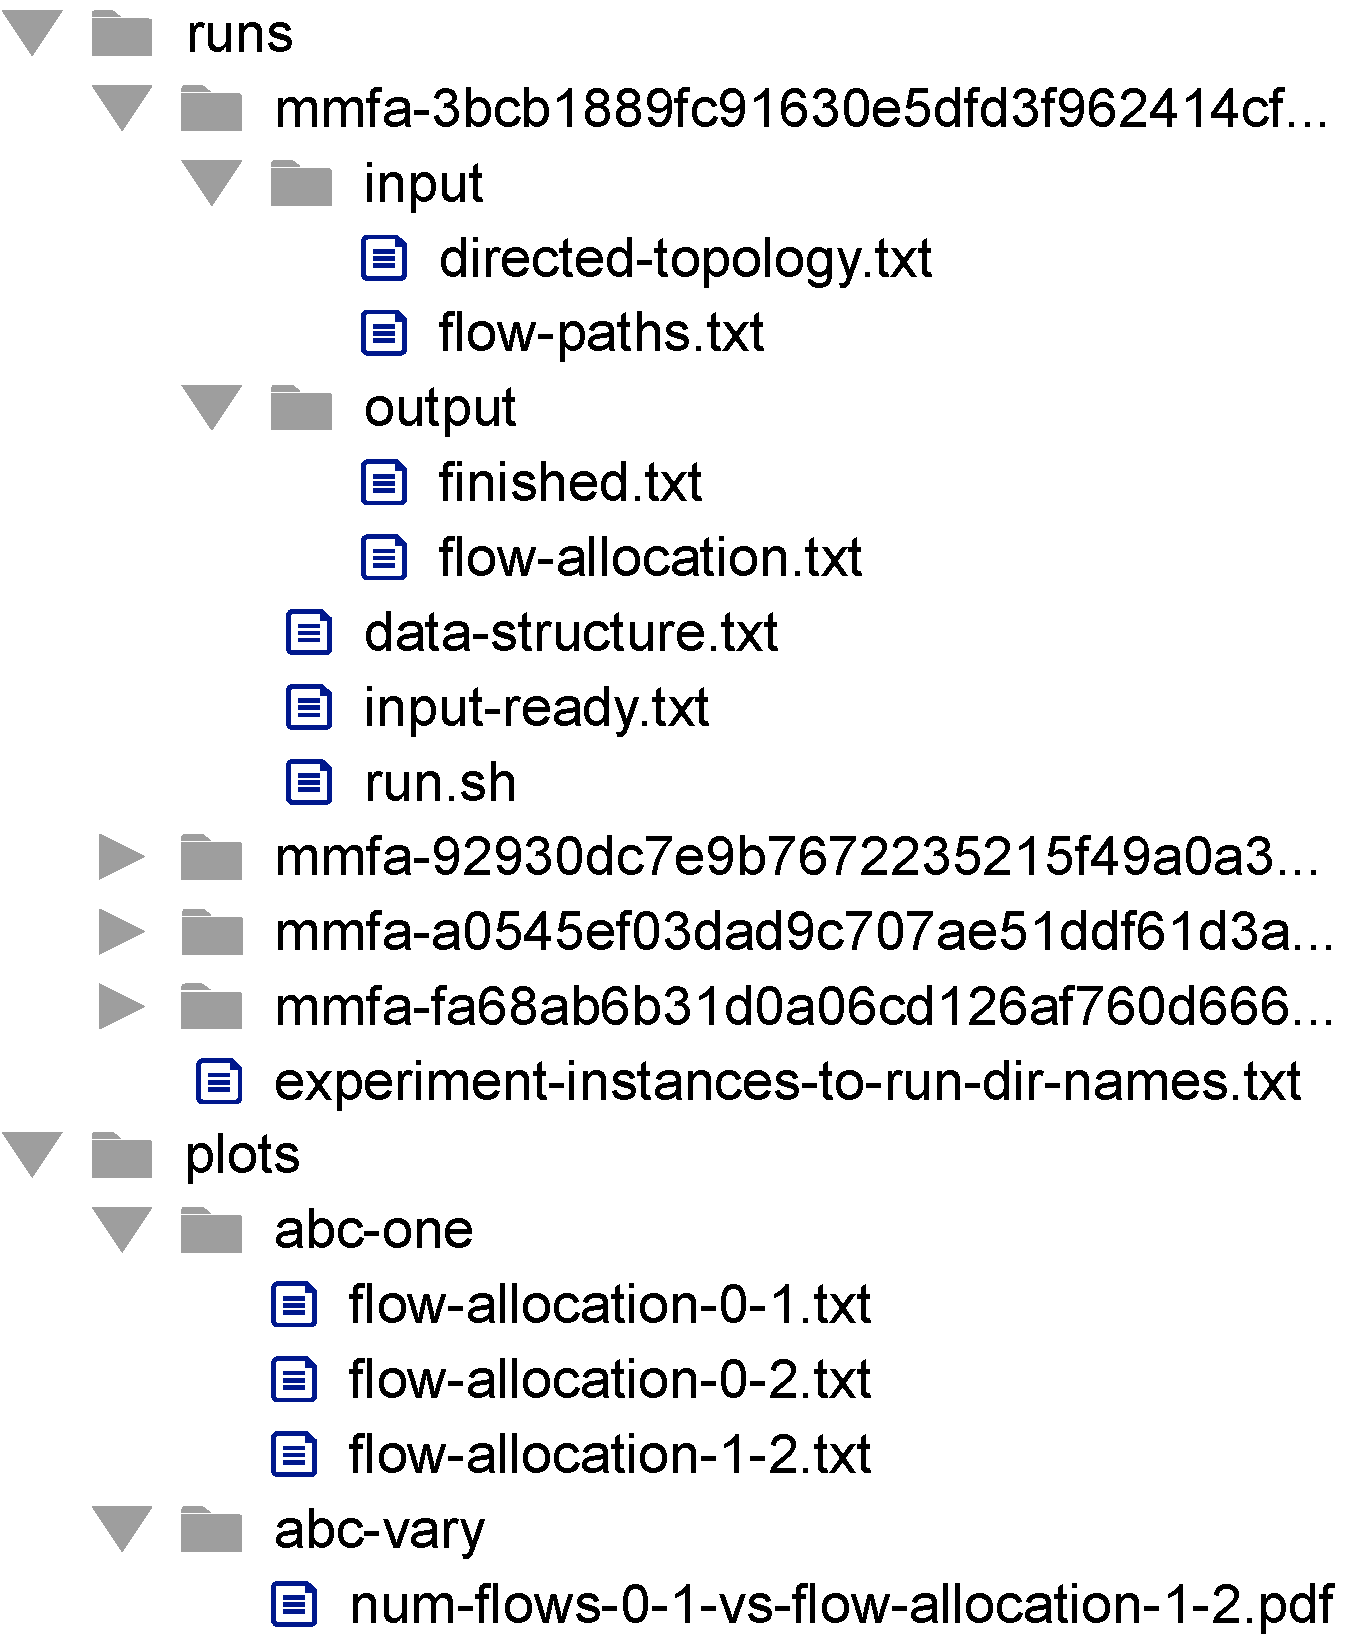
\includegraphics[width=0.35\textwidth]{figures/runs-plots.pdf}
\caption{Runs, plots folders of the max-min fairness example.}
\label{fig:runs}
\vspace{-6pt}
\end{figure}

\parab{Task 4: generate run script for each run directory}\\
As its final task, the interpreter generates a bash execution script, \textit{run.sh}, for each run folder. In its \textit{run.sh} script, it should call on its run framework to process the input, and output its logs into the run directory. After the interpret phase for all root classes finishes, our current implementation walks sequentially through the runs directory, executing each \textit{run.sh} file. Of course, this can also be done using a more sophisticated job scheduler, \eg to accommodate parallel executions.

For our max-min fairness example, running the \textit{run.sh} in a directory first checks whether the output folder already contains a \textit{finished.txt} file indicating if this run was already executed. Otherwise, it uses Python to execute a max-min fair allocation solver, the input to which are the paths to the run's input and output directories. (The implemented max-min fair allocation algorithm is based on section II.B of \cite{nace2006} and uses networkx~\cite{networkx} for graph data structures.)

%%%%%%%%%%%%%%%%%%%%%%%%%%%%%%%%%%%%%%%%%%%%%%%%%%%%%%
%%%%%%%%%%%%%%%%%%%%%%%%%%%%%%%%%%%%%%%%%%%%%%%%%%%%%%
%%%%%%%%%%%%%%%%%%%%%%%%%%%%%%%%%%%%%%%%%%%%%%%%%%%%%%
%%%%%%%%%%%%%%%%%%%%%%%%%%%%%%%%%%%%%%%%%%%%%%%%%%%%%%
%%%%%%%%%%%%%%%%%%%%%%%%%%%%%%%%%%%%%%%%%%%%%%%%%%%%%%

\subsection{Plotter: consume logs, produce results}
\label{sec:plotter}

For each root class, authors build a post-processing pipeline. 

\begin{itemize}[leftmargin=12pt,itemsep=2pt,topsep=2pt]
    \item From the parser, the plotter learns which plot files to generate for each experiment instance, as declared through \texttt{\textbackslash expincludetext} and \texttt{\textbackslash expincludegraphics}.
    
    \item From the interpreter it learns which run directories exist for each experiment instance by reading \textit{experiment-instances-to-run-dir-names.txt}.
    
    \item For each experiment instance, it creates a directory in the \textit{plots} directory in which it places the output plot files.
    
    \item For each experiment instance, it goes over the list of plot files and generates them one after the other. A plot file can use both experiment input and output data.
    
\end{itemize}

\noindent For our running example, we can generate the following files from processing the experiment results:

\begin{itemize}[leftmargin=12pt,itemsep=2pt,topsep=2pt]
    \item \textit{flow-allocation-(from)-(to).txt} : Amount allocated to each flow between the from and to nodes, without trailing zeroes. Such files are only generated for an experiment instance which maps to a single run directory.
    \item \textit{num-flows-(from)-(to)-vs-flow-allocation-(src)-(dst).pdf} : 2D plot, with the $x$-axis being the number of flows between the \textit{from} and \textit{to} nodes, and the $y$-axis being the amount of flow allocated to each flow from \textit{src} to \textit{dst}.
\end{itemize}

%%%%%%%%%%%%%%%%%%%%%%%%%%%%%%%%%%%%%%%%%%%%%%%%%%%%%%
%%%%%%%%%%%%%%%%%%%%%%%%%%%%%%%%%%%%%%%%%%%%%%%%%%%%%%
%%%%%%%%%%%%%%%%%%%%%%%%%%%%%%%%%%%%%%%%%%%%%%%%%%%%%%
%%%%%%%%%%%%%%%%%%%%%%%%%%%%%%%%%%%%%%%%%%%%%%%%%%%%%%
%%%%%%%%%%%%%%%%%%%%%%%%%%%%%%%%%%%%%%%%%%%%%%%%%%%%%%

\subsection{Final product: PDF generation}

After all the promised output plot files have been generated, the \texttt{\textbackslash expincludetext} and \texttt{\textbackslash expincludegraphics} commands will include the promised resources into the paper correctly. A standard \LaTeX{} compilation pipeline with, \eg pdflatex and bibtex, suffices to generate the paper. To this end, we make use of TeX Live~\cite{texlive}.

\section{Guidance for authors}
\label{sec:guidance-for-authors}

To maintain its applicability to a variety of experiment types, \sysname is designed to function as scaffolding for the authors' experiment framework(s). Authors use the simple \experimentex markup in their \LaTeX{} writeup, and implement two additional components besides their usual experiment framework(s): interpreters and plotters. These are just hooks to run-scripts and post-processing routines authors would write anyway, but nevertheless, based on our experience using \sysname, we offer guidance for authors for using \experimentex markup and for writing interpreters and plotters.

\subsection{Writing order and strategy}
\label{sec:writing-strategy}

\begin{enumerate}[leftmargin=12pt,itemsep=2pt,topsep=2pt]
    \item Consider which types of experiments (\textit{expclasses}) will exist, and what their relevant parameters are;
    \item Consider which concrete experiments (\textit{expinstances}) will be run, and if they have overlaps that could benefit from defining shared \textit{expclasses} to inherit from;
    \item Envelop the sentences which describe the experiment setup, such as parameters, with \textit{explines};
    \item Represent text (\eg words, metrics) which depends on experimental results using \textit{expincludetext} commands;
    \item Represent figures which depend on experimental results using \textit{expincludegraphics} commands.
\end{enumerate}

\noindent Once authors have an initial draft, they can start with implementing an interpreter and plotter. They can then continue iterating, cycling between: (a) writing new text with new or modified explines and expincludes; (b) extending the interpreter to incorporate the explines; (c) extending the plotter to be able to satisfy the new expincludes; and potentially also (d) extending or adding running frameworks.

\subsection{Best practices}
\label{sec:best-practices}

We formulate the following design principles to guide authors towards productive use of \sysname:

\begin{itemize}[leftmargin=10pt,itemsep=2pt,topsep=2pt]
    \item For transparency and consistency, make runs self-contained, using input configuration files only in the run directory.
    \item For determinism and reproducibility, control randomness via seed parameters. For conducting multiple runs for statistical confidence, a list of seed attributes can be used.
    \item To maximize interactivity for readers, expose any parameters and settings that may influence the results via \textit{explines}. Explines should be intuitive and easy to edit, and not overly sensitive to whitespace, capitalization, punctuation, etc.
    \item For consistency of the writeup, use \textit{expincludes} for all possible result values in text, and for result plots.
    \item Use \LaTeX{} comments around markup to indicate acceptable values for parameters, options for system configuration, which result metrics / plots can be generated, etc.
\end{itemize}


\noindent \sysname does not preclude the use of collaborative online \LaTeX{} editors, but using it in this setting requires that at least one author additionally use an environment that can run \sysname and the authors' experiment frameworks, and manually upload the generated output files. This inconvenience could be overcome by a future extended collaborative editing service that additionally uses cloud resources to enable \sysname on the same platform.

\begin{figure*}[t]
	\centering
	\hspace*{\fill}%
	\subfigure[TCP Cubic]{%
		\label{fig:cc:together-cubic}%
		\expincludegraphics[width=2.3in]{tcp-cubic}{plot_tcp_flow_time_vs_together_0.pdf}%
	}%
	\hfill%
	\subfigure[TCP Vegas]{%
		\label{fig:cc:together-vegas}%
		\expincludegraphics[width=2.3in]{tcp-vegas}{plot_tcp_flow_time_vs_together_0.pdf}%
	}%
	\hfill%
	\subfigure[DCTCP]{%
		\label{fig:cc:together-dctcp}%
		\expincludegraphics[width=2.3in]{tcp-dctcp}{plot_tcp_flow_time_vs_together_0.pdf}%
	}%
	\hspace*{\fill}\vspace{-2pt}%
	\caption{\small \em Various TCP state variables over time for each of the congestion control protocols.}%\
	\label{fig:cc:together}
	\vspace{-6pt}
\end{figure*}

\begin{figure*}[t]
	\centering%
	\hspace*{\fill}%
	\subfigure[TCP Cubic]{%
		\label{fig:cc:rate-cubic}%
		\expincludegraphics[width=2.3in]{tcp-cubic}{plot_tcp_flow_time_vs_rate_0.pdf}%
	}%
	\hfill%
	\subfigure[TCP Vegas]{%
		\label{fig:cc:rate-vegas}%
		\expincludegraphics[width=2.3in]{tcp-vegas}{plot_tcp_flow_time_vs_rate_0.pdf}%
	}%
	\hfill%
	\subfigure[DCTCP]{%
		\label{fig:cc:rate-dctcp}%
		\expincludegraphics[width=2.3in]{tcp-dctcp}{plot_tcp_flow_time_vs_rate_0.pdf}%
	}%
	\hspace*{\fill}\vspace{-2pt}%
	\caption{\small \em Achieved rate over time for each of the congestion control protocols.}
	\label{fig:cc:rate}
	\vspace{-6pt}
\end{figure*}

\begin{figure*}[t]
	\centering
	\hspace*{\fill}%
	\subfigure[TCP Cubic]{%
		\label{fig:cc:rtt-cubic}%
		\expincludegraphics[width=2.3in]{tcp-cubic}{plot_tcp_flow_time_vs_rtt_0.pdf}%
	}%
	\hfill%
	\subfigure[TCP Vegas]{%
		\label{fig:cc:rtt-vegas}%
		\expincludegraphics[width=2.3in]{tcp-vegas}{plot_tcp_flow_time_vs_rtt_0.pdf}%
	}%
	\hfill%
	\subfigure[DCTCP]{%
		\label{fig:cc:rtt-dctcp}%
		\expincludegraphics[width=2.3in]{tcp-dctcp}{plot_tcp_flow_time_vs_rtt_0.pdf}%
	}%
	\hspace*{\fill}\vspace{-2pt}%
	\caption{\small \em Measured round-trip time (RTT) over time for each of the congestion control protocols.}
	\label{fig:cc:rtt}
	\vspace{-6pt}
\end{figure*}

\section{Showcase 1: congestion control}
\label{sec:congestion-control}

Congestion control protocols are designed to work in a wide range of network settings. However, in some circumstances they perform better than in others, \eg due to assumptions on delay or loss. For readers to gain a deeper understanding of congestion control protocols being proposed, they should be able to both vary the network settings as well as the parameters of the protocols. To this end, we present a simple scenario for which we investigate how various commonly known TCP variants perform. It gives the readers a direct way to interact with congestion control protocols and test their hypotheses -- without having to first be exposed to the code base of the underlying adaptation of the ns-3 packet-level simulator~\cite{ns3} with the basic-sim module~\cite{basic-sim}. All of the following experiments, in this showcase and the following two, are \sysname generated, so interested readers can tinker with them.

\subsection{Experimental setup}
\expclass{cc-one}{one-link-tcp}
\parab{Topology.} We use a single link topology with two nodes.
% One can edit the runtime in seconds.
% E.g., another possibility: The experiment is run for 5~seconds.
\expline{cc-one}{The experiment is run for 20~seconds.}
% One can edit all the number values
% E.g., another possibility: The link has the following properties: the channel has a delay of 90~ms, and its network devices have a data rate of 10~Mbit/s, 0.3\% random packet loss, and a FIFO queue of 32 packets.
\expline{cc-one}{The link has the following properties: the channel has a delay of 20~ms, and its network devices have a data rate of 20~Mbit/s, 0.001\% random packet loss, and a FIFO queue of 50 packets.}
% One can edit the queue size and the marking threshold.
% E.g., another possibility: We set a random early detection (RED) queueing discipline with a maximum queue size of 45 packets and a binary marking (or drop if the IP packet does not support ECN) threshold at 20 packets.
\expline{cc-one}{We set a random early detection (RED) queueing discipline with a maximum queue size of 100 packets and a binary marking (or drop if the IP packet does not support ECN) threshold at 50 packets.}

\parab{Transport protocol.} We start a single uni-directional long-lasting TCP connection from the first node to the second. The init congestion window is \expline[init-cwnd-pkt]{cc-one}{10}, and the segment size \expline[segment-size]{cc-one}{1380~byte} (MTU is 1500 byte). The timestamp option is \expline[opt-timestamp]{cc-one}{enabled}, SACK is \expline[opt-sack]{cc-one}{enabled}, and window scaling is \expline[opt-win-scaling]{cc-one}{enabled}. No-delay (as in, disabling Nagle's algorithm) is \expline[no-delay]{cc-one}{enabled}. Pacing is \expline[opt-pacing]{cc-one}{disabled}. To increase the accuracy of RTT measurements, \expline{cc-one}{delayed acknowledgements are disabled}. The timing settings are as follows: maximum segment lifetime is set to \expline[max-seg-lifetime]{cc-one}{1~s}, minimum RTO to \expline[min-rto]{cc-one}{200~ms}, initial RTT estimate to \expline[initial-rtt-estimate]{cc-one}{400~ms}, connection timeout to \expline[connection-timeout]{cc-one}{400~ms}, and persist timeout to \expline[persist-timeout]{cc-one}{800~ms}. \expline{cc-one}{The send and receive buffer size are set to 1~GB} such that there is sufficient data available to accommodate large congestion windows.\footnote{Naturally, a long list of all parameters involved can make for tiresome reading. Authors can decide if certain parameters are completely irrelevant and omit them entirely from the text; however, they must weigh the risk that readers do not agree with the authors' omissions.}

\subsection{Results}

\expinstance{tcp-cubic}{cc-one}
\noindent\textbf{\expline{tcp-cubic}{TCP Cubic}} is a loss-based protocol; packets will be dropped when the combined queue size of the network device (\expincludetext{tcp-cubic}{ndq-size-pkt.txt}) and the threshold of the RED queuing discipline (\expincludetext{tcp-cubic}{qdisc-threshold-pkt.txt}) on top of the bandwidth delay product are exceeded (\expincludetext{tcp-cubic}{bdp-pkt.txt}). As such, each time the congestion window reaches around \expincludetext{tcp-cubic}{ndq-qdisc-bdp-pkt.txt} in Fig.~\ref{fig:cc:together-cubic}, a loss occurs and the congestion window is cut. TCP Cubic achieves an average rate of \expincludetext{tcp-cubic}{average-rate-Mbps.txt}~Mbit/s, and an average RTT of \expincludetext{tcp-cubic}{average-rtt-ms.txt}~ms.

\expinstance{tcp-vegas}{cc-one}
\parab{\expline{tcp-vegas}{TCP Vegas}.} TCP Vegas is a delay-based protocol, and will only grow its congestion window if it does not increase RTT. Thus, if the congestion window is larger than the bandwidth-delay product (\expincludetext{tcp-vegas}{bdp-pkt.txt}), the congestion window will not grow as it would increase the RTT due to additional queueing delay (see Fig.~\ref{fig:cc:together-vegas}). TCP Vegas achieves an average rate of \expincludetext{tcp-vegas}{average-rate-Mbps.txt}~Mbit/s, and an average RTT of \expincludetext{tcp-vegas}{average-rtt-ms.txt}~ms.

\expinstance{tcp-dctcp}{cc-one}
\parab{\expline{tcp-dctcp}{DCTCP}.} It makes clever use of marked early congestion notifications (ECN) to limit the amount of queueing it causes in the network. As a consequence, it maintains the same queue size and does not do the aggressive reductions as exhibited by TCP Cubic. Its congestion window as such hovers around \expincludetext{tcp-dctcp}{ndq-qdisc-bdp-pkt.txt} (see Fig.~\ref{fig:cc:together-dctcp}). DCTCP achieves an average rate of \expincludetext{tcp-dctcp}{average-rate-Mbps.txt}~Mbit/s, and an average RTT of \expincludetext{tcp-dctcp}{average-rtt-ms.txt}~ms.

\greybox{\textbf{Behind the scenes:} In the LaTeX source code all the network settings are editable (\eg channel delay, device data rate, ...). If you change their values in the LaTeX and execute the reproduce pipeline, all the figures (Fig.~\ref{fig:cc:together}, \ref{fig:cc:rate} and \ref{fig:cc:rtt}) and all the metrics mentioned in-text (\eg bandwidth-delay product, average rate, average RTT, ...) will be automatically updated.}


\begin{figure*}[t]

    %%%%%%%%%%%%%%%%%%%%%%%%%%%%%%%
    % CODEBIND HELP NOTES
    %
    % For each of the below figures, the format is as follows:
    % plot_target_load_vs_tcp_flows_[small/large]_fct_ns_[statistic].pdf
    % OR:
    % plot_target_load_vs_tcp_flows_[small/large]_avg_throughput_megabit_per_s_[statistic].pdf
    %
    % With [statistic] can be any of the following:
    % min
    % 0_1th
    % 1th
    % 10th
    % median
    % mean
    % 90th
    % 99th
    % 99_9th
    % max
    %
    
	\centering
	\hspace*{\fill}%
	\subfigure[Average FCT]{%
		\label{fig:netload:small:average-fct}%
		\expincludegraphics[width=1.75in]{load-ls-main}{plot_target_load_vs_tcp_flows_small_fct_ns_average.pdf}%
	}%
	\hfill%
	\subfigure[99th \%-tile FCT]{%
		\label{fig:netload:small:99th-fct}%
		\expincludegraphics[width=1.75in]{load-ls-main}{plot_target_load_vs_tcp_flows_small_fct_ns_99th_percentile.pdf}%
	}%
	\hfill%
	\subfigure[Average throughput]{%
		\label{fig:netload:small:average-rate}%
		\expincludegraphics[width=1.75in]{load-ls-main}{plot_target_load_vs_tcp_flows_small_avg_throughput_megabit_per_s_average.pdf}%
	}%
	\hfill%
	\subfigure[1th \%-tile throughput]{%
		\label{fig:netload:small:1th-rate}%
		\expincludegraphics[width=1.75in]{load-ls-main}{plot_target_load_vs_tcp_flows_small_avg_throughput_megabit_per_s_1th_percentile.pdf}%
	}%
	\hspace*{\fill}\vspace{-4pt}%
	\caption{\small \em Performance of the small TCP flows. Each line point is the average of the metric across runs, the vertical bar around it are the minimum and maximum.}
	\label{fig:netload:small}
	\vspace{4pt}%

	\hspace*{\fill}%
	\subfigure[Average FCT]{%
		\label{fig:netload:large:average-fct}%
		\expincludegraphics[width=1.75in]{load-ls-main}{plot_target_load_vs_tcp_flows_large_fct_ns_average.pdf}%
	}%
	\hfill%
	\subfigure[99th \%-tile FCT]{%
		\label{fig:netload:large:99th-fct}%
		\expincludegraphics[width=1.75in]{load-ls-main}{plot_target_load_vs_tcp_flows_large_fct_ns_99th_percentile.pdf}%
	}%
	\hfill%
	\subfigure[Average throughput]{%
		\label{fig:netload:large:average-rate}%
		\expincludegraphics[width=1.75in]{load-ls-main}{plot_target_load_vs_tcp_flows_large_avg_throughput_megabit_per_s_average.pdf}%
	}%
	\hfill%
	\subfigure[1th \%-tile throughput]{%
		\label{fig:netload:large:1th-rate}%
		\expincludegraphics[width=1.75in]{load-ls-main}{plot_target_load_vs_tcp_flows_large_avg_throughput_megabit_per_s_1th_percentile.pdf}%
	}%
	\hspace*{\fill}\vspace{-4pt}%
	\caption{\small \em Performance of the large TCP flows. Each line point is the average of the metric across runs, the vertical bar around it are the minimum and maximum.}
	\label{fig:netload:large}
	\vspace{-6pt}
\end{figure*}

\section{Showcase 2: DC experiments}
\label{sec:netload}

\expinstance{load-ls-main}{load-ls}
Next, instead of focusing on a single connection as in \S\ref{sec:congestion-control}, we evaluate the performance of an entire network using ns-3~\cite{ns3} with the basic-sim module~\cite{basic-sim}. We want to show the network performance for a workload consisting of a mix of small and large flows. We want to make a comparison between two settings: one in which all flows are treated equal, and the other in which the small flows are prioritized absolutely over the large flows

\parab{Network topology.} The network is a leaf-spine topology, in which each leaf is connected to every spine. The leaves are top-of-rack (ToR) switches which connect each to a set of servers. \expline{load-ls-main}{There are 2 spines and 3 leaves.} \expline{load-ls-main}{Each leaf (ToR) has 3 servers underneath.} \expline{load-ls-main}{Every link has the following properties: the channel has a delay of 20~$\mu s$, and its network devices have a data rate of 100~Mbit/s, 0.001\% random packet loss, and a FIFO queue of 5 packets.} \expline{load-ls-main}{We set pfifo\_fast as the queueing discipline with a maximum total queue size of 200 packets.}

\parab{Transport protocol.} \expline{load-ls-main}{We set TCP Cubic as the congestion control protocol.} The initial congestion window is set to \expline[init-cwnd-pkt]{load-ls-main}{10}, and the segment size to \expline[segment-size]{load-ls-main}{1380~byte} (MTU is 1500 byte). The timestamp option is \expline[opt-timestamp]{load-ls-main}{enabled}, SACK option is \expline[opt-sack]{load-ls-main}{enabled}, and window scaling is \expline[opt-win-scaling]{load-ls-main}{enabled}. No-delay (as in, disabling Nagle's algorithm) is \expline[no-delay]{load-ls-main}{enabled}. Pacing is \expline[opt-pacing]{load-ls-main}{disabled}. To increase the accuracy of RTT measurements, \expline{load-ls-main}{delayed acknowledgements are disabled}. The timing settings are as follows: maximum segment lifetime is set to \expline[max-seg-lifetime]{load-ls-main}{1~s}, minimum RTO to \expline[min-rto]{load-ls-main}{200~ms}, initial RTT estimate to \expline[initial-rtt-estimate]{load-ls-main}{400~ms}, connection timeout to \expline[connection-timeout]{load-ls-main}{400~ms}, and persist timeout to \expline[persist-timeout]{load-ls-main}{800~ms}. \expline{load-ls-main}{The send and receive buffer size are set to 1~GB} such that there is sufficient data available to accommodate large congestion windows.\footnote{To avoid the redundancy in the text here, which is similar to the previous showcase, we could use inheritance from the same class. For this paper, we wanted to keep the showcases self-contained, so we did not take this route.}

\parab{Workload.} The workload consists of uni-directional TCP flows, and is modeled after the approach of HULL~\cite{hull}, albeit with a simpler Bernoulli flow size distribution. We use a Poisson process to determine the inter-arrival rate $\lambda$. For each flow, the source and destination server are chosen uniformly at random. \expline{load-ls-main}{The flow size is randomly chosen to be either small (50~KB) with 90\% probability, or large (4~MB) with 10\% probability.} Under the all-to-all traffic pattern, the leaf-spine network becomes bottlenecked most optimistically at \expincludetext{load-ls-main}{bottleneck-Mbps.txt}~Mb/s. We model target load with respect to this bottleneck limit by expressing the target load as a fraction of it. \expline{load-ls-main}{We vary the target load from 5\% till 60\% in increments of 5\%.} With the used flow size distribution (with mean flow size \expincludetext{load-ls-main}{mean-flow-size.txt}), this equates to varying the Poisson flow arrival rate $\lambda$ from \expincludetext{load-ls-main}{lambda-lowest.txt}~flow/s till \expincludetext{load-ls-main}{lambda-highest.txt}~flow/s in approximate steps of \expincludetext{load-ls-main}{lambda-step.txt}~flow/s. \expline{load-ls-main}{Only the flows which start in the measurement period are included in the result: the flows which started in the warm-up period of the first 5~seconds and the cool-down period of the last 20~seconds are not taken into account.} \expline{load-ls-main}{The experiment is configured such that in expectation 4000 flows start in the measurement period.} However, of those, only the flows which finished were incorporated in the result as it is undefined what the FCT for an incomplete flow is. \expline{load-ls-main}{Each load point is run for 5 times, with a reproducible initial random seed based on the (SHA-256) hash of its unique run configuration.}

%%%%%%%%%%%%%%%%%%%%%%%%%%%%%%%
% CODEBIND HELP NOTES
%
% Expincludes:
%
% Format:  lambda-[load].txt
% Example: lambda-10.txt
% Prints:  Flow arrival rate in flows/s
%
% DIRECT VALUES
% ---
%
% Format:  load-[load]-[equal/prioritized]-[all/small/large]-fct-[statistic].txt
% Example: load-20-equal-vs-prioritized-all-fct-max.txt
% Prints:  Speed-up
%
% Format:  load-[load]-[equal/prioritized]-[all/small/large]-throughput-[statistic].txt
% Example: load-20-equal-all-throughput-max.txt
% Prints:  Speed-up
%
% Format:  load-[load]-[equal/prioritized]-[server-leaf/leaf-spine]-utilization-[statistic].txt
% Example: load-20-equal-leaf-spine-utilization-max.txt
%
% FOR A CERTAIN LOAD, SPEED-UP OF EQUAL VS. PRIORITIZED
% ---
%
% Format:  load-[load]-[equal/prioritized]-vs-[equal/prioritized]-[all/small/large]-fct-[statistic].txt
% Example: load-20-equal-vs-prioritized-all-fct-max.txt
% Prints:  Speed-up
%
% Format:  load-[load]-[equal/prioritized]-vs-[equal/prioritized]-[all/small/large]-throughput-[statistic].txt
% Example: load-20-equal-vs-prioritized-all-throughput-max.txt
% Prints:  Speed-up
%
% Format:  load-[load]-[equal/prioritized]-vs-[equal/prioritized]-[server-leaf/leaf-spine]-utilization-[statistic].txt
% Example: load-20-equal-vs-prioritized-leaf-spine-utilization-max.txt
% Prints:  Increase ("speed-up")
%
% FOR A CERTAIN EQUAL OR PRIORITIZED, SPEED-UP ACROSS LOADS
% ---
%
% Format:  load-[loadA]-vs-loadB]-[equal/prioritized]-[all/small/large]-fct-[statistic].txt
% Example: load-20-vs-30-equal-all-fct-max.txt
% Prints:  Speed-up
%
% Format:  load-[loadA]-vs-loadB]-[equal/prioritized]-[all/small/large]-throughput-[statistic].txt
% Example: load-20-vs-30-prioritized-all-throughput-max.txt
% Prints:  Speed-up
%
% Format:  load-[loadA]-vs-loadB]-[equal/prioritized]-[server-leaf/leaf-spine]-utilization-[statistic].txt
% Example: load-20-vs-30-prioritized-leaf-spine-utilization-max.txt
% Prints:  Increase ("speed-up")
%
% With [statistic] can be any of the following:
% min
% 0-1th
% 1th
% 10th
% median
% mean
% 90th
% 99th
% 99-9th
% max
%

\parab{Small flows are significantly sped up.} The small flows complete in a few round-trips. However, if their packets get stuck behind packets of larger flows, this can drastically increase flow completion time. By prioritizing these small flows (given they only take up \expincludetext{load-ls-main}{small-flow-size-total-percentage.txt}\% of the total bytes), their performance drastically improves. At 10\% target load, prioritized small flows achieve a speed-up factor of \expincludetext{load-ls-main}{load-10-equal-vs-prioritized-small-fct-average.txt}$\times$ on average FCT and \expincludetext{load-ls-main}{load-10-equal-vs-prioritized-small-fct-99th-percentile.txt}$\times$ at the 99th \%-tile FCT. At higher target loads, the speed-up becomes even more apparent (see Fig.~\ref{fig:netload:small}).

\parab{Large flows are not impacted much.} The large flows make up the bulk of the total workload bytes (\expincludetext{load-ls-main}{large-flow-size-total-percentage.txt}\%). The large flows are \expincludetext{load-ls-main}{large-flow-size-divided-small-flow-size.txt}$\times$ larger than that of their smaller workload counterparts, and as such, there are significantly fewer of them (\expincludetext{load-ls-main}{ratio-small-large-flows.txt}). Because of their size, they require many round-trips to complete, and are present longer in the network. All these factors combined lighten the impact if one prioritizes small flows over them. At 10\% target load, the prioritization of small flows only causes on average a speedup of the large flows of \expincludetext{load-ls-main}{load-10-equal-vs-prioritized-large-fct-average.txt}$\times$ on average FCT and \expincludetext{load-ls-main}{load-10-equal-vs-prioritized-large-fct-99th-percentile.txt}$\times$ at the 99th \%-tile FCT. (Speedup below one implies slowdown.)

\parab{FCT vs. throughput.} There is an inverse relationship between FCT and rate. As such, there is a direct relationship between $x$th \%-tile FCT and $(100 - x)$th \%-tile rate (see Fig.~\ref{fig:netload:large:99th-fct}/\ref{fig:netload:large:1th-rate}). However, it is a non-linear function, as such there is no linear relationship between the average FCT and the average rate (see Fig.~\ref{fig:netload:large:average-fct}/\ref{fig:netload:large:average-rate}).

\parab{Network performance degrades near saturation.} The workload is a product of three random processes which (by design) do not spread perfectly. The target flow arrival rate only guarantees that it averages out over time. However, as the arrival rate approaches the service rate of the network (the total bandwidth given the traffic pattern), the flow completion time will increase more. In the equal priority setting, increasing the load from 10\% to 30\% results in a \expincludetext{load-ls-main}{load-10-vs-30-equal-all-fct-average.txt}$\times$ speedup for the large flow average FCT, whereas increasing from 30\% to 50\% results in a \expincludetext{load-ls-main}{load-30-vs-50-equal-all-fct-average.txt}$\times$ speedup. The cool-down period of \expincludetext{load-ls-main}{cool-down-s.txt}~s is crucial to be able to take into account even the slowest of large flow completions. This is shown by the near 100\% completion fraction across flows for all loads in Fig.~\ref{fig:netload:completed}.

\begin{figure}
    %%%%%%%%%%%%%%%%%%%%%%%%%%%%%%%
    % CODEBIND HELP NOTES
    %
    % For each of the below figures, the format is as follows:
    % plot_target_load_vs_tcp_flows_[small/large]_fraction_completed.pdf
    %
    \centering%
    \hspace*{\fill}%
    \subfigure[Small flows]{%
        \label{fig:netload:completed:small}%
        \expincludegraphics[width=1.65in]{load-ls-main}{plot_target_load_vs_tcp_flows_small_fraction_completed.pdf}%
    }%
    \hfill%
    \subfigure[Large flows]{%
        \label{fig:netload:completed:large}%
        \expincludegraphics[width=1.65in]{load-ls-main}{plot_target_load_vs_tcp_flows_large_fraction_completed.pdf}%
    }%
    \hspace*{\fill}\vspace{-3pt}%
    \caption{\small \em Amount of both types of flows which were completed.}%
    \label{fig:netload:completed}%
    \vspace{-7pt}%
\end{figure}

\parab{Target load vs. actual load.} The aforementioned bottleneck (\expincludetext{load-ls-main}{bottleneck-Mbps.txt}~Mb/s) against which we normalize target load is very optimistic for 3 reasons: (a) it does not account for additionally header and acknowledgement overhead, which adds additional load beyond that of payload; (b) the load is a result of three random processes and as such can lead to hot spots causing the network to be saturated earlier; and (c) TCP and ECMP are not always able to take full advantage of the network's capacity. To illustrate this, in Fig.~\ref{fig:netload:utilization:server-leaf} and Fig.~\ref{fig:netload:utilization:leaf-spine} we show the utilization of the server-leaf and leaf-spine links. At $\lambda=\expincludetext{load-ls-main}{lambda-40.txt}\text{~flows/s}$ the target load is 40\%, but the \textit{average} maximum link utilization is \expincludetext{load-ls-main}{load-40-equal-server-leaf-utilization-max.txt}\% (server-leaf) and \expincludetext{load-ls-main}{load-40-equal-leaf-spine-utilization-max.txt}\% (leaf-spine).

\begin{figure}
    %%%%%%%%%%%%%%%%%%%%%%%%%%%%%%%
    % CODEBIND HELP NOTES
    %
    % For each of the below figures, the format is as follows:
    % plot_target_load_vs_[server_leaf/leaf_spine]_link_utilization_fraction_[statistic].pdf
    %
    % With [statistic] can be any of the following:
    % min
    % 0_1th
    % 1th
    % 10th
    % median
    % mean
    % 90th
    % 99th
    % 99_9th
    % max
    %
	\centering
	\hspace*{\fill}%
	\subfigure[Server-leaf links]{%
		\label{fig:netload:utilization:server-leaf}%
		\expincludegraphics[width=1.65in]{load-ls-main}{plot_target_load_vs_server_leaf_link_utilization_fraction_max.pdf}%
	}%
	\hfill%
	\subfigure[Leaf-spine links]{%
		\label{fig:netload:utilization:leaf-spine}%
		\expincludegraphics[width=1.65in]{load-ls-main}{plot_target_load_vs_leaf_spine_link_utilization_fraction_max.pdf}%
	}%
	\hspace*{\fill}\vspace{-3pt}%
	\caption{\small \em Network utilization as the workload intensifies.}
	\label{fig:netload:utilization}
	\vspace{-7pt}
\end{figure}

\greybox{\textbf{Behind the scenes:} In the LaTeX source code it is possible to up or down scale the size of the network, as well as vary the load put upon it. However, as one increases the scale or load, the experiments will take longer to complete. Both the workload characteristics as well as the performance metrics (\eg FCT, throughput, ...) are automatically updated based on the experimental setup defined.}

\begin{figure*}[t]
    
    %%%%%%%%%%%%%%%%%%%%%%%%%%%%%%%
    % CODEBIND HELP NOTES
    %
    % For each of the below figures, the format is as follows:
    % plot-rank-against-daily-change-[statistic].pdf
    %
    % With [statistic] can be any of the following:
    % min
    % mean
    % max
    % median
    % percentile-X with X in {0, 1, 2, ..., 100}
    %
    
	\centering
% 	\hspace*{\fill}%
	\subfigure[Mean]{%
		\label{fig:toplists:mean}%
		\expincludegraphics[width=2.3in]{tl}{plot-rank-against-daily-change-mean.pdf}%
	}%
	\hfill%
	\subfigure[10th \%-tile]{%
		\label{fig:toplists:10th}%
		\expincludegraphics[width=2.3in]{tl}{plot-rank-against-daily-change-percentile-10.pdf}%
	}%
 	\hfill%
	\subfigure[90th\%-tile]{%
		\label{fig:toplists:90th}%
		\expincludegraphics[width=2.3in]{tl}{plot-rank-against-daily-change-percentile-90.pdf}%
	}%
% 	\hspace*{\fill}
	\vspace{-2pt}%
	\caption{\small \em Various daily change metrics across the top-K of Internet top domain lists (data from Fig.~2(c) of \cite{top-lists}).}
	\label{fig:toplists}
	\vspace{-6pt}
\end{figure*}

\expinstance{tl}{top-lists}
\section{Showcase 3: Dataset Analysis}
\label{sec:dataset-analysis}

Not all experiments can be reproduced by readers --- the code might be proprietary, the hardware used might be custom, or it might be prohibitively expensive to rent the computational power needed for it to finish in feasible time. It is also possible that the experiments are inherently the result of a manual process (\eg a questionnaire), or a process which is not easily repeatable. As such, it is not possible to have the readers tweak the experimental setup. However, instead, authors can expose the dataset, and permit readers to interactively explore the dataset beyond what is shown in the paper.

We use the dataset and accompanying code made publicly available by Scheitle et al.~\cite{top-lists}. In their work, they analyze 3 commonly used ranked lists of Web domains: Alexa (Alexa-18 referring to using data from end of January 2018 till April 2018, and Alexa-1318 to data from 2013 till end of January 2018), Umbrella, and Majestic. The study characterizes, compares, and explains the differences of these lists. Their core experiment was the daily download of these lists over a long period of time, which they subsequently used to investigate how they evolved over time.

We focus on a small part of their study in which they analyze how stable the top lists are on a daily basis (\S6.1 of \cite{top-lists}). In it, they want to investigate whether, \eg the top-100 domains are more stable than the top-1000. For every list, they calculate from the lists what percent of the top-K has changed on each day. They use the mean across days as the metric, and graphically plot it against rank (Fig.~\ref{fig:toplists:mean}). The mean daily change of the top-1K and top-10K for Alexa-18 are respectively \expincludetext{tl}{alexa-18-daily-change-rank-1000-mean.txt} and \expincludetext{tl}{alexa-18-daily-change-rank-10000-mean.txt}, whereas for Umbrella-JOINT they are \expincludetext{tl}{umbrella-joint-daily-change-rank-1000-mean.txt} and \expincludetext{tl}{umbrella-joint-daily-change-rank-10000-mean.txt}. In the mean, Alexa-18 is the most unstable top list for top-1K and top-10k.

An inquisitive reader might be interested in statistics beyond the mean, for instance to understand better the best of daily changes look like (\eg its 10th percentile), or conversely the worst cases (\eg its 90th percentile). With \sysname the authors can empower the reader to be able to easily add additional plots to find out (Fig.~\ref{fig:toplists:10th} and Fig.~\ref{fig:toplists:90th}).

\parab{Worst daily changes.} The 90th percentile daily change of the top-1K and top-10K for Alexa-18 are \expincludetext{tl}{alexa-18-daily-change-rank-1000-percentile-90.txt} and \expincludetext{tl}{alexa-18-daily-change-rank-10000-percentile-90.txt}, whereas for Umbrella-JOINT they are respectively \expincludetext{tl}{umbrella-joint-daily-change-rank-1000-percentile-90.txt} and \expincludetext{tl}{umbrella-joint-daily-change-rank-10000-percentile-90.txt}. In this instance, the reader is able to observe that for the top-1K and especially the top-10K, Umbrella-JOINT's 10\% of worst days are similar to those of Alexa-18.

\parab{Best vs. worst daily changes.} The 10th percentile for Umbrella-JOINT is significantly better than its 90th percentile: the top-1M sees \expincludetext{tl}{umbrella-joint-daily-change-rank-1000000-percentile-10.txt} daily change vs. \expincludetext{tl}{umbrella-joint-daily-change-rank-1000000-percentile-90.txt}. For Alexa-18 on the other hand, this difference is not as large: its top-1M sees \expincludetext{tl}{alexa-18-daily-change-rank-1000000-percentile-10.txt} vs. \expincludetext{tl}{alexa-18-daily-change-rank-1000000-percentile-90.txt} at its 10th and 90th percentile. The extremities of daily change proportionally vary more for Umbrella-JOINT than for Alexa-18.

All of above are additional observations that can help the reader to gain a deeper understanding of the paper's subject matter. Further, if the reader has even more specific questions whose metrics and plots are not present in the plotter, the reader at least has a starting point to trace the plots that are there to their origins in the code base.

\greybox{\textbf{Behind the scenes:} In cases where readers cannot feasibly rerun the experiments, \sysname still adds value: authors can use it to empower readers to explore plots beyond those shown in the paper, as well as to extract data point values directly from plots.}

\section{Which networking papers can benefit from \sysname?}\vspace{4pt}

We examined all $65$ NSDI-2020 papers to assess which ones could benefit from \sysname. A tabulation with greater detail is available in Appendix~\ref{appendix:nsdianalysis}, but in summary:

\begin{itemize}[leftmargin=10pt,itemsep=2pt,topsep=2pt]

    \item $38$ papers ($58\%$) have parameters or experimental settings that could be interesting for readers to tweak.
    
    \item $23$ papers ($35\%$) make use of general compute to perform computation, simulation or emulation experiments. Of these, \textbf{14 papers (22\%)} have parameters or experimental settings that could be interesting for readers to tweak.
    
    \item $19$ papers ($29\%$) make use public cloud infrastructure to run system deployment experiments. Of these, \textbf{17 papers (26\%)} have parameters readers may want to tinker with.
    
    \item \textbf{5 papers (8\%)} have a significant focus on a data set, which \sysname can help expose to readers in a more engaging, interactive manner.
    
\end{itemize}

\noindent In all, \textbf{18 papers (28\%)} could directly benefit from the features of \sysname, engaging readers in modifying experiment settings or/and in exploring substantial datasets. If authors automate cloud experiments and readers have access to cloud infrastructure to run such experiments, 30 papers (46\%) could benefit. Further, even for the work that depends on bespoke testbeds, \sysname-enabled papers allow readers to dive deeper into the experimental results.

\section{Reproducibility with \sysname}
\label{sec:pipeline}

\sysname enables reproducibility, such that: (a) the paper's text drives the author-supplied experiment code to regenerate the paper's results; and (b) the code corresponding to the results and text is easier to identify. Publication venues can also use it to \emph{enforce} reproducibility if desired, as follows.

The authors submit two artifacts: the paper PDF and the code base. The code base comprises the paper's \LaTeX{} source, all experiment code, and two scripts: (1) \textit{setup\_env.sh}, which can recreate the authors' environment from scratch; and (2) \textit{reproduce.sh}, which can run the \sysname pipeline to regenerate the paper. Publication venues can archive pre-built environments produced from running \textit{setup\_env.sh}, if desirable, to guard against the code becoming obsolete due to evolution of the software dependencies in the environment.

To ensure integrity, the two artifacts above can be irrevocably linked: the paper should include a pointer to the code base, together with a checksum across the code base in the paper's text. In the code base's copy of the paper \LaTeX{}, this checksum is set to zeroes to avoid a cyclic dependency. For our paper, this information is in the footnote on page 1.

The reproducibility of a paper can be evaluated by comparing the output PDF from \sysname used on the environment built from scratch, to the authors' submitted document.  One can also evaluate what fraction of a paper is reproducible in a manner similar to how software projects evaluate coverage by test cases, using a continuous integration and delivery (CI/CD) methodology~\cite{redhat-ci-cd}. Mock-ups of what such a reproducibility evaluation might output are included in Appendix~\ref{appendix:reproducibility}.

\section{\sysname's limitations}
\label{sec:limitations}

\sysname is a substantial step in improving the correctness, reproducibility, and usefulness of networking papers. Nevertheless, it has several limitations:

\begin{itemize}[leftmargin=10pt,itemsep=2pt,topsep=2pt]

    \item Not all experiments are easy to rerun, \eg due to custom hardware or constraints on runtime and resources needed. Cloud providers sponsoring resources to support reproducibility for top networking conferences could help, but ultimately, authors must carefully select which experiment setups to expose to readers with \sysname. Note that even for hard-to-rerun experiments, expincludes are still beneficial, as authors can expose different facets of their results, and allow readers to customize the data analysis.
    
    \item For some experiments, variance stems from real world artifacts. For instance, recent work revealed the performance variability in public cloud environments~\cite{nsdi-2020-uta}. Authors should convey what counts as a successful reproduction of their results by explicitly noting the expected range of variations, and thus set reader expectations accordingly. (This should be standard practice in any case.)
    
    \item Naturally, even a \sysname-enabled paper's readers are only limited to the experiments the authors frame and expose. Auto-generated plots may also have visual artifacts, which authors often adjust for manually in the particular results included. To overcome such problems, \sysname can be seen as an entry point for readers to engage with the authors' code through the interpreters and plotters.
    
    \item Authors draw conclusions and write descriptive text beyond just result metrics. When readers change experiments using \sysname, it is non-trivial for authors to have code in place to modify such text descriptions. \sysname can be seen as an attempt to push authors to draw conclusions robust to a variety of plausible experiment settings, but readers must also be forgiving of textual descriptions that do not tightly match the readers' tweaked experiments, especially for extreme parameter settings.
    
    \item \sysname only removes one source of inconsistencies and errors, namely those resulting from independent, manual evolution of experiments and their writing. Of course, the authors' run-scripts or other parts of their code-base can still contain bugs that \sysname does not help against.

\end{itemize}

\section{Alternative approaches}
\label{sec:alternative-approaches}

\sysname allows authors to retain complete freedom in designing their experiments, while still providing a way to directly couple them with the paper document. We believe it to be unique in these capabilities.

\textbf{Online websites}, which some authors build to accompany papers, can indeed allow even greater interactivity. Despite the sizable burden this imposes on authors, this approach still does not help with the issue of ensuring consistency between a paper's text/plots and the experiments behind them. While we chose to work within the bounds of today's dominant \LaTeX{}-generated-PDF mode of publishing networks research, a best-of-both-worlds approach could use a \sysname-like approach with HTML markup (and visible user-interface elements for editing the editable parts) instead of \LaTeX{} markup.

It is also possible to \textbf{insert code/scripts in LaTeX~\cite{pythontex, pynea, bar2020reproduciblelatex}}. But this requires readers to understand the code, which can be difficult for  complex experiment pipelines. Another similar idea is that of using a meta-programming language to compile to \LaTeX{}~\cite{orgmode}, but this just moves the problem to understanding the meta-programming language. These solutions would also shift the content and writing style of papers substantially, and would likely impair readability and meet resistance from both authors and reviewers / readers.

\textbf{Jupyter notebooks}~\cite{jupyter-notebooks} enable interactive code, with accompanying text, and result visuals. The intended interaction mode is for readers to edit the code, while \sysname's intent is to \textit{not} require that, and instead, to have most readers think of code as a blackbox, for which they can change inputs and select the outputs. (A subset of readers may use \sysname's hooks to the code as entry points for deeper examination.) Further, Jupyter notebooks do not address the issue of separation between paper-text and system-experiments that \sysname addresses, and are limited to self-contained experiments using a few select language runtimes, far short of the diversity of experiment methods used in networking papers.

\textbf{Gigaleaf}~\cite{gigaleaf} is a platform which synchronizes the plots from a Jupyter notebook into a \LaTeX{} folder. It is however only one-way: it is not possible to have the \LaTeX{} text control which experiments to run or which results to create.

\section{Conclusion}
\label{sec:conclusion}

We introduced \sysname, a system for authors to: (a) expose configurable parts of their experiments to readers in an easy-to-use manner; and (b) enforce consistency between their paper and its underlying experiments. With the addition of simple and minimally obtrusive mark-up to its \LaTeX{} source, the paper's text itself controls the experiments. This enables readers to interact with the text and understand the behavior of the involved systems under different inputs, \textit{without} needing any knowledge of the underlying system code. 

We showed \sysname in action across three types of experiments: using \textit{congestion control} and \textit{data center} experiments, we showed \sysname's utility in allowing readers to tweak the large number of parameters and knobs in such experiments; and using a \textit{dataset analysis} example, we showed that even when readers cannot rerun some experiments, they can still benefit from unprecedented interactivity with the data presented in the paper. We also showed \sysname's utility in the teaching of networking concepts, with an illustration on \textit{max-min fairness} that allows students to learn the concept deeply by interacting with the example.

This paper is itself written using \sysname. A video demo of \sysname, using parts of this paper, is \href{https://drive.google.com/file/d/1U_3MxQ84FaE8fkTME6MF_SFuZIRhzTnv/view}{available online}. The code base for this paper is linked on page 1, and \textbf{we encourage readers to themselves modify the \LaTeX{} code in \S\ref{sec:example}, \S\ref{sec:congestion-control}, \S\ref{sec:netload}, and \S\ref{sec:dataset-analysis} to see how the text and results change in place.} \sysname presents a way forward for authors to make their work more consistent, reproducible, and transparent to readers.\footnote{Another potential benefit of \sysname is in accessibility: for readers who are visually-impaired, having a system like \sysname could enable them to interactively explore texts with the aid of text-to-speech tools. This can reduce the barrier they might face otherwise in extracting information from the graphical elements that typically summarize results in papers. However, this is not something we have been able to get feedback on yet.}


\clearpage

\bibliographystyle{ACM-Reference-Format}
\bibliography{bibliography}

\appendix
\section{Example: what it looks like if you compile like normal}
\label{sec:compile-like-normal}

If one would skip the \sysname pipeline and directly compile the \LaTeX{} from the example in \S\ref{sec:example} (\ie using pdflatex, bibtex), it produces placeholders for the unavailable expincludes:

\vspace{0.2cm}
% %%%%%%%%%%%%%%%%%%%%%%%%%%%%%%%%%%%%%%%%%%%%%%%%%%%%%%%%%
% NOTE: the underneath LaTeX does not have any \expinclude... commands, because it is just to showcase what would happen if one would not execute the CodeBind pipeline beforehand. If we would use expincludes with either incorrect experiment names or incorrect filenames here, the pipeline would throw an error when going over this section.
\begin{mdframed}[style=annotex]

Under max-min fairness, the addition of flows to the network can \emph{increase} the throughput of some flows.

To demonstrate this, we use a simple topology of three nodes with two directed edges:
the edge from A to B has a capacity of 1 unit,
and the the edge from B to C has a capacity of 1 unit.

In the first experiment, we start the following flows: one from A to B (path is A$\rightarrow$B), one from B to C (path is B$\rightarrow$C), and one from A to C (path is A$\rightarrow$B$\rightarrow$C).
This results in a max-min fair allocation of \textbf{\textcolor{red}{[\texttt{X}]}}, \textbf{\textcolor{red}{[\texttt{X}]}} and \textbf{\textcolor{red}{[\texttt{X}]}} for each type respectively.

\begin{center}
% Source file: figures/topology-example.drawio

\includegraphics[width=3cm]{figures/topology-example.pdf}
\end{center}

However, say we increase the number of flows from A to B. What would happen to the flow from B to C? In the second experiment, as before we start one flow from B to C and one flow from A to C. We vary the number of flows from A to B between 1 and 4. The addition of extra flows from A to B results in the flow from A to C being bottlenecked there, resulting in the flow from B to C being allocated more.

\begin{center}
\includegraphics[width=4.7cm]{example-image-a}
\end{center}

\end{mdframed}
% %%%%%%%%%%%%%%%%%%%%%%%%%%%%%%%%%%%%%%%%%%%%%%%%%%%%%%%%%

%%%%%%%%%%%%%%%%%%%%%%%%%%%%%%%%%%%%%%%%%%%%
%%%%%%%%%%%%%%%%%%%%%%%%%%%%%%%%%%%%%%%%%%%%
%%%%%%%%%%%%%%%%%%%%%%%%%%%%%%%%%%%%%%%%%%%%
%%%%%%%%%%%%%%%%%%%%%%%%%%%%%%%%%%%%%%%%%%%%
%%%%%%%%%%%%%%%%%%%%%%%%%%%%%%%%%%%%%%%%%%%%

\section{Publication venue reproducibility pipeline}
\label{appendix:reproducibility}

An overview of the publication venue reproducibility pipeline is depicted in Fig.~\ref{fig:venue-reproducibility-pipeline}. The authors supply the two artifacts, and the CI/CD pipeline spins up a fresh start container, clones the code base into it, and executes the \textit{setup\_env.sh} and \textit{reproduce.sh} scripts. Venue should store the container both after successful completion of \textit{setup\_env.sh} and after \textit{reproduce.sh} to safeguard against \eg dependency evolution or fallout. Although the first container should have the entire environment setup, the second container is stored in the eventuality of there mistakenly being an external dependency being retrieved by the \textit{reproduce.sh} script. The generated PDF would be compared against the submitted PDF for any differences, and a report could be generated as a result for both authors and reviewers (see Fig.~\ref{fig:reproducibility-checker} and \ref{fig:paper-pdf-delta}).

\parab{Code base pointer and checksum.} We define one extra command: \texttt{\textbackslash expcodechecksum\{\}} prints the code checksum. It import the value from the \textit{code-checksum.txt} file within the paper \LaTeX{} folder. The checksum of the code base is either (a) if it was supplied as a single file archive, its (SHA-256) hash, or (b) if it is a git repository, its git commit hash. Authors first finalize their code base and determine the checksum. Afterwards, they run their code one more time with the correct code checksum to generate the PDF to submit -- it is never committed to the code base. The code checksum must be set to zeroes in the code base (to prevent a cyclic dependency). The reproducibility submission system would similarly calculate or retrieve the checksum from the submitted code base, and insert it before starting the code base execution.

The authors must place the following piece of \LaTeX{} in their paper:

\vspace{0.2cm}
\begin{mdframed}[style=annotex]
\begin{verbatim}
This paper is written using CodeBind.
\url{https://venue.com/year/paper-name}
Code checksum: \expcodechecksum{}
\end{verbatim}
\end{mdframed}

\noindent If the submission system permits authors to supply supplemental archives, the URL can potentially be left out while the paper is under submission though must be included in the camera-ready.

\begin{figure}
    % Source file: figures/venue-reproducibility-pipeline.key
    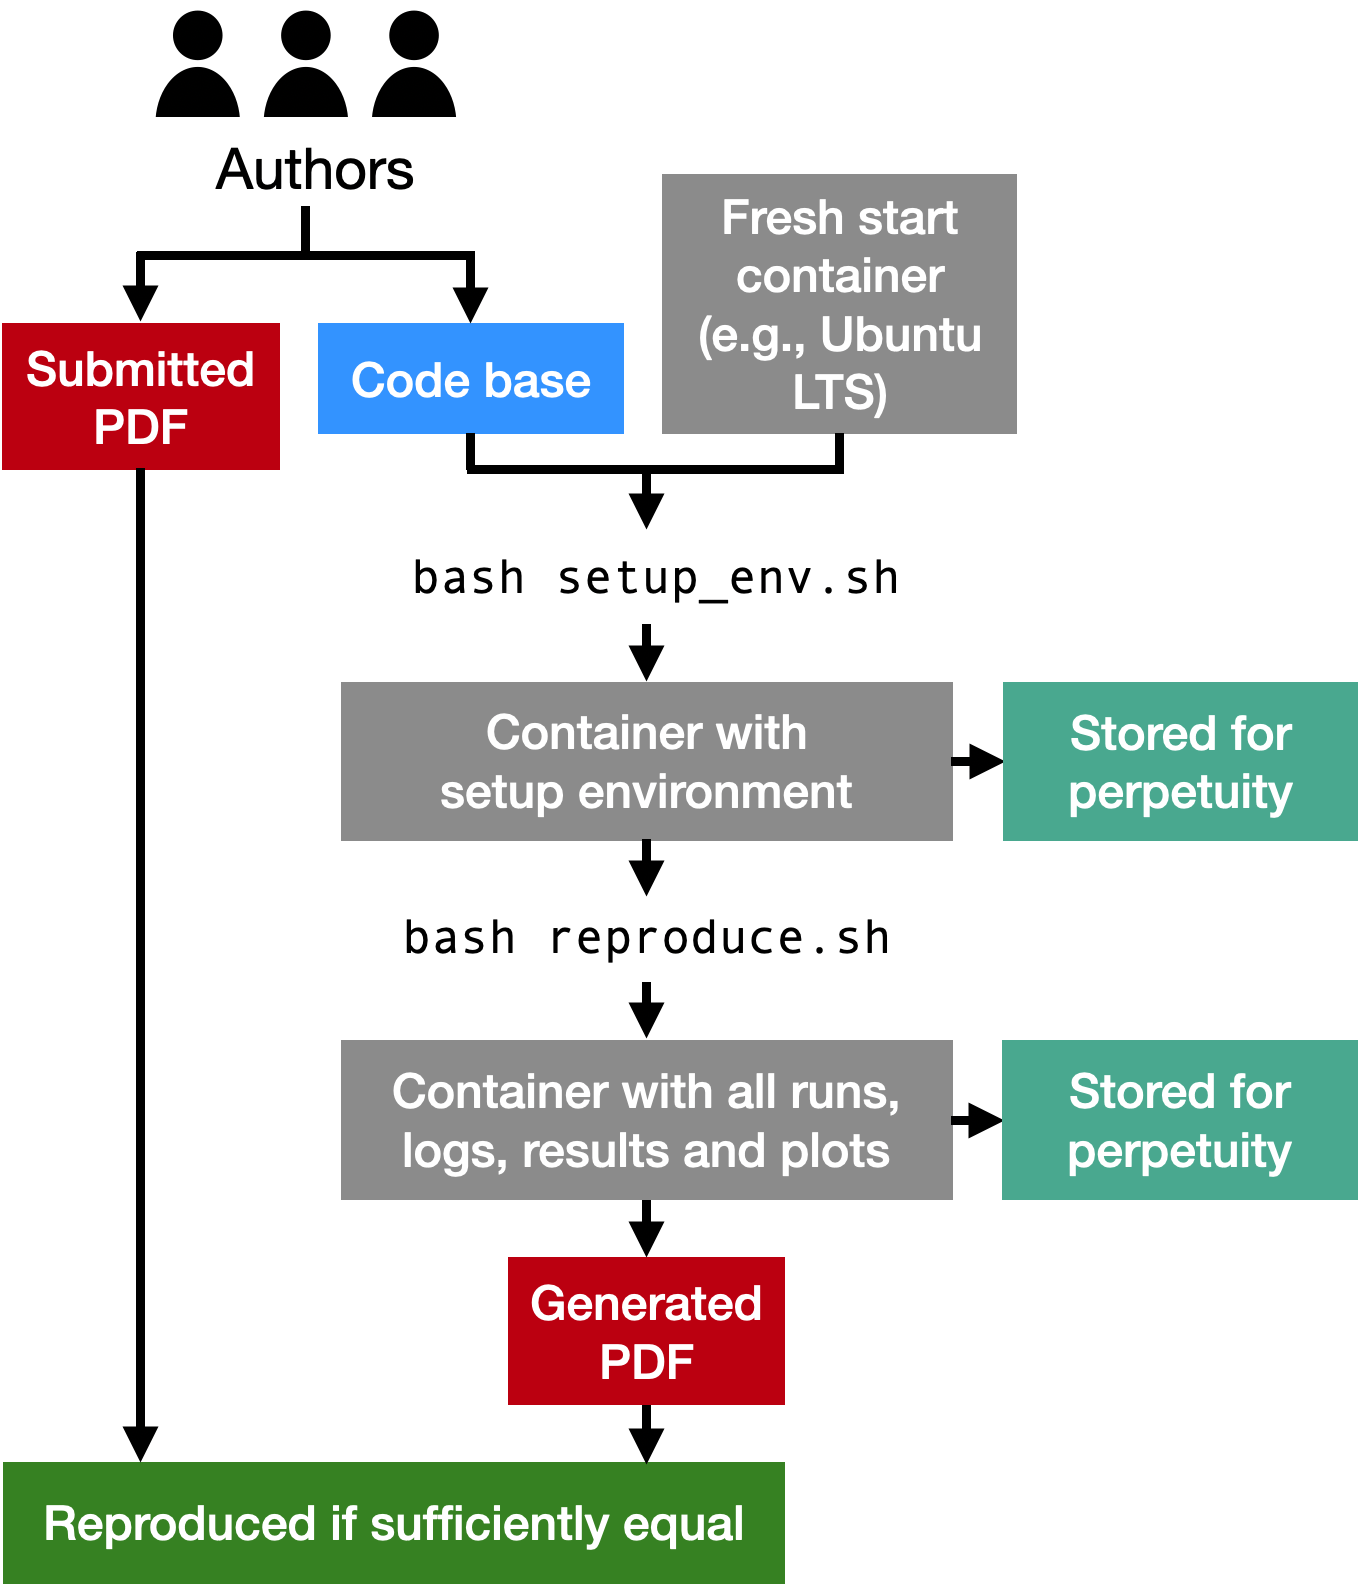
\includegraphics[width=0.48\textwidth]{figures/venue-reproducibility-pipeline.png}
    \caption{Overview of a pipeline a publication venue could use to enforce reproducibility.}
    \label{fig:venue-reproducibility-pipeline}
\end{figure}

\begin{figure}
    % Source file: figures/reproducibility-checker.key
    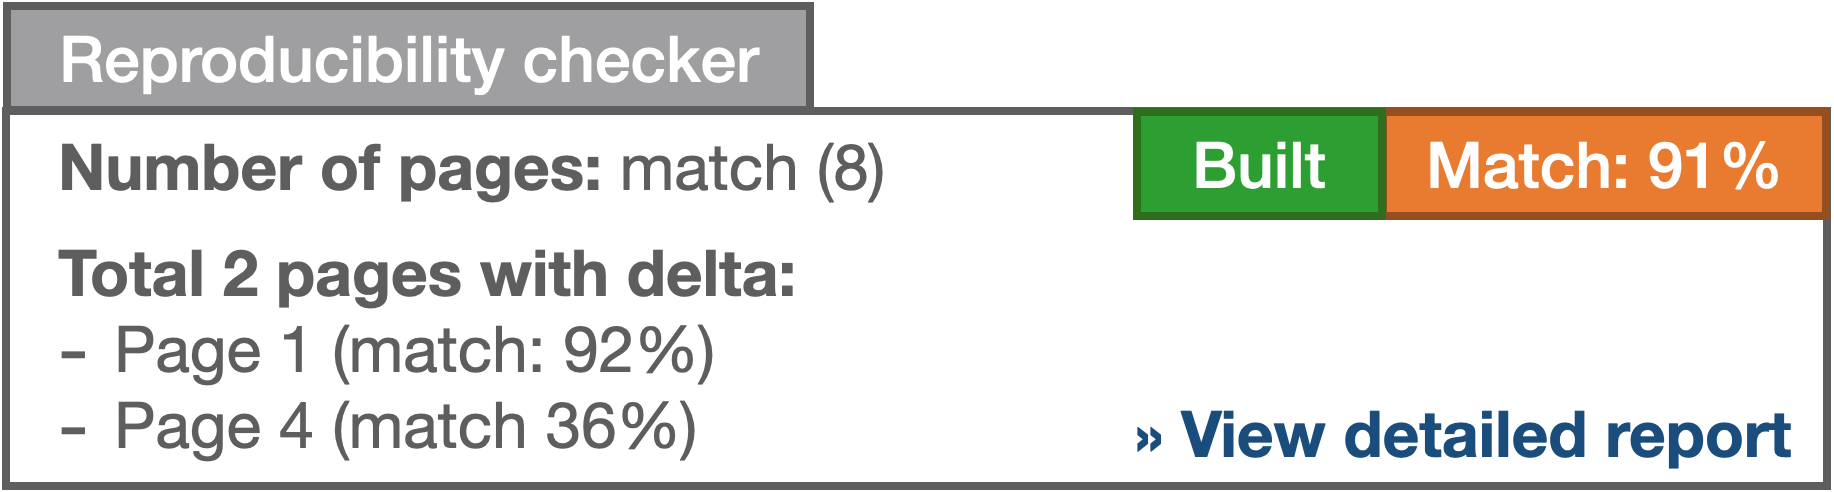
\includegraphics[width=0.48\textwidth]{figures/reproducibility-checker.png}
    \caption{Similar to the format checker in HotCRP, we propose the reproducibility checker (mock-up).}
    \label{fig:reproducibility-checker}
\end{figure}

\begin{figure}
    % Source file: figures/paper-pdf-delta.drawio
    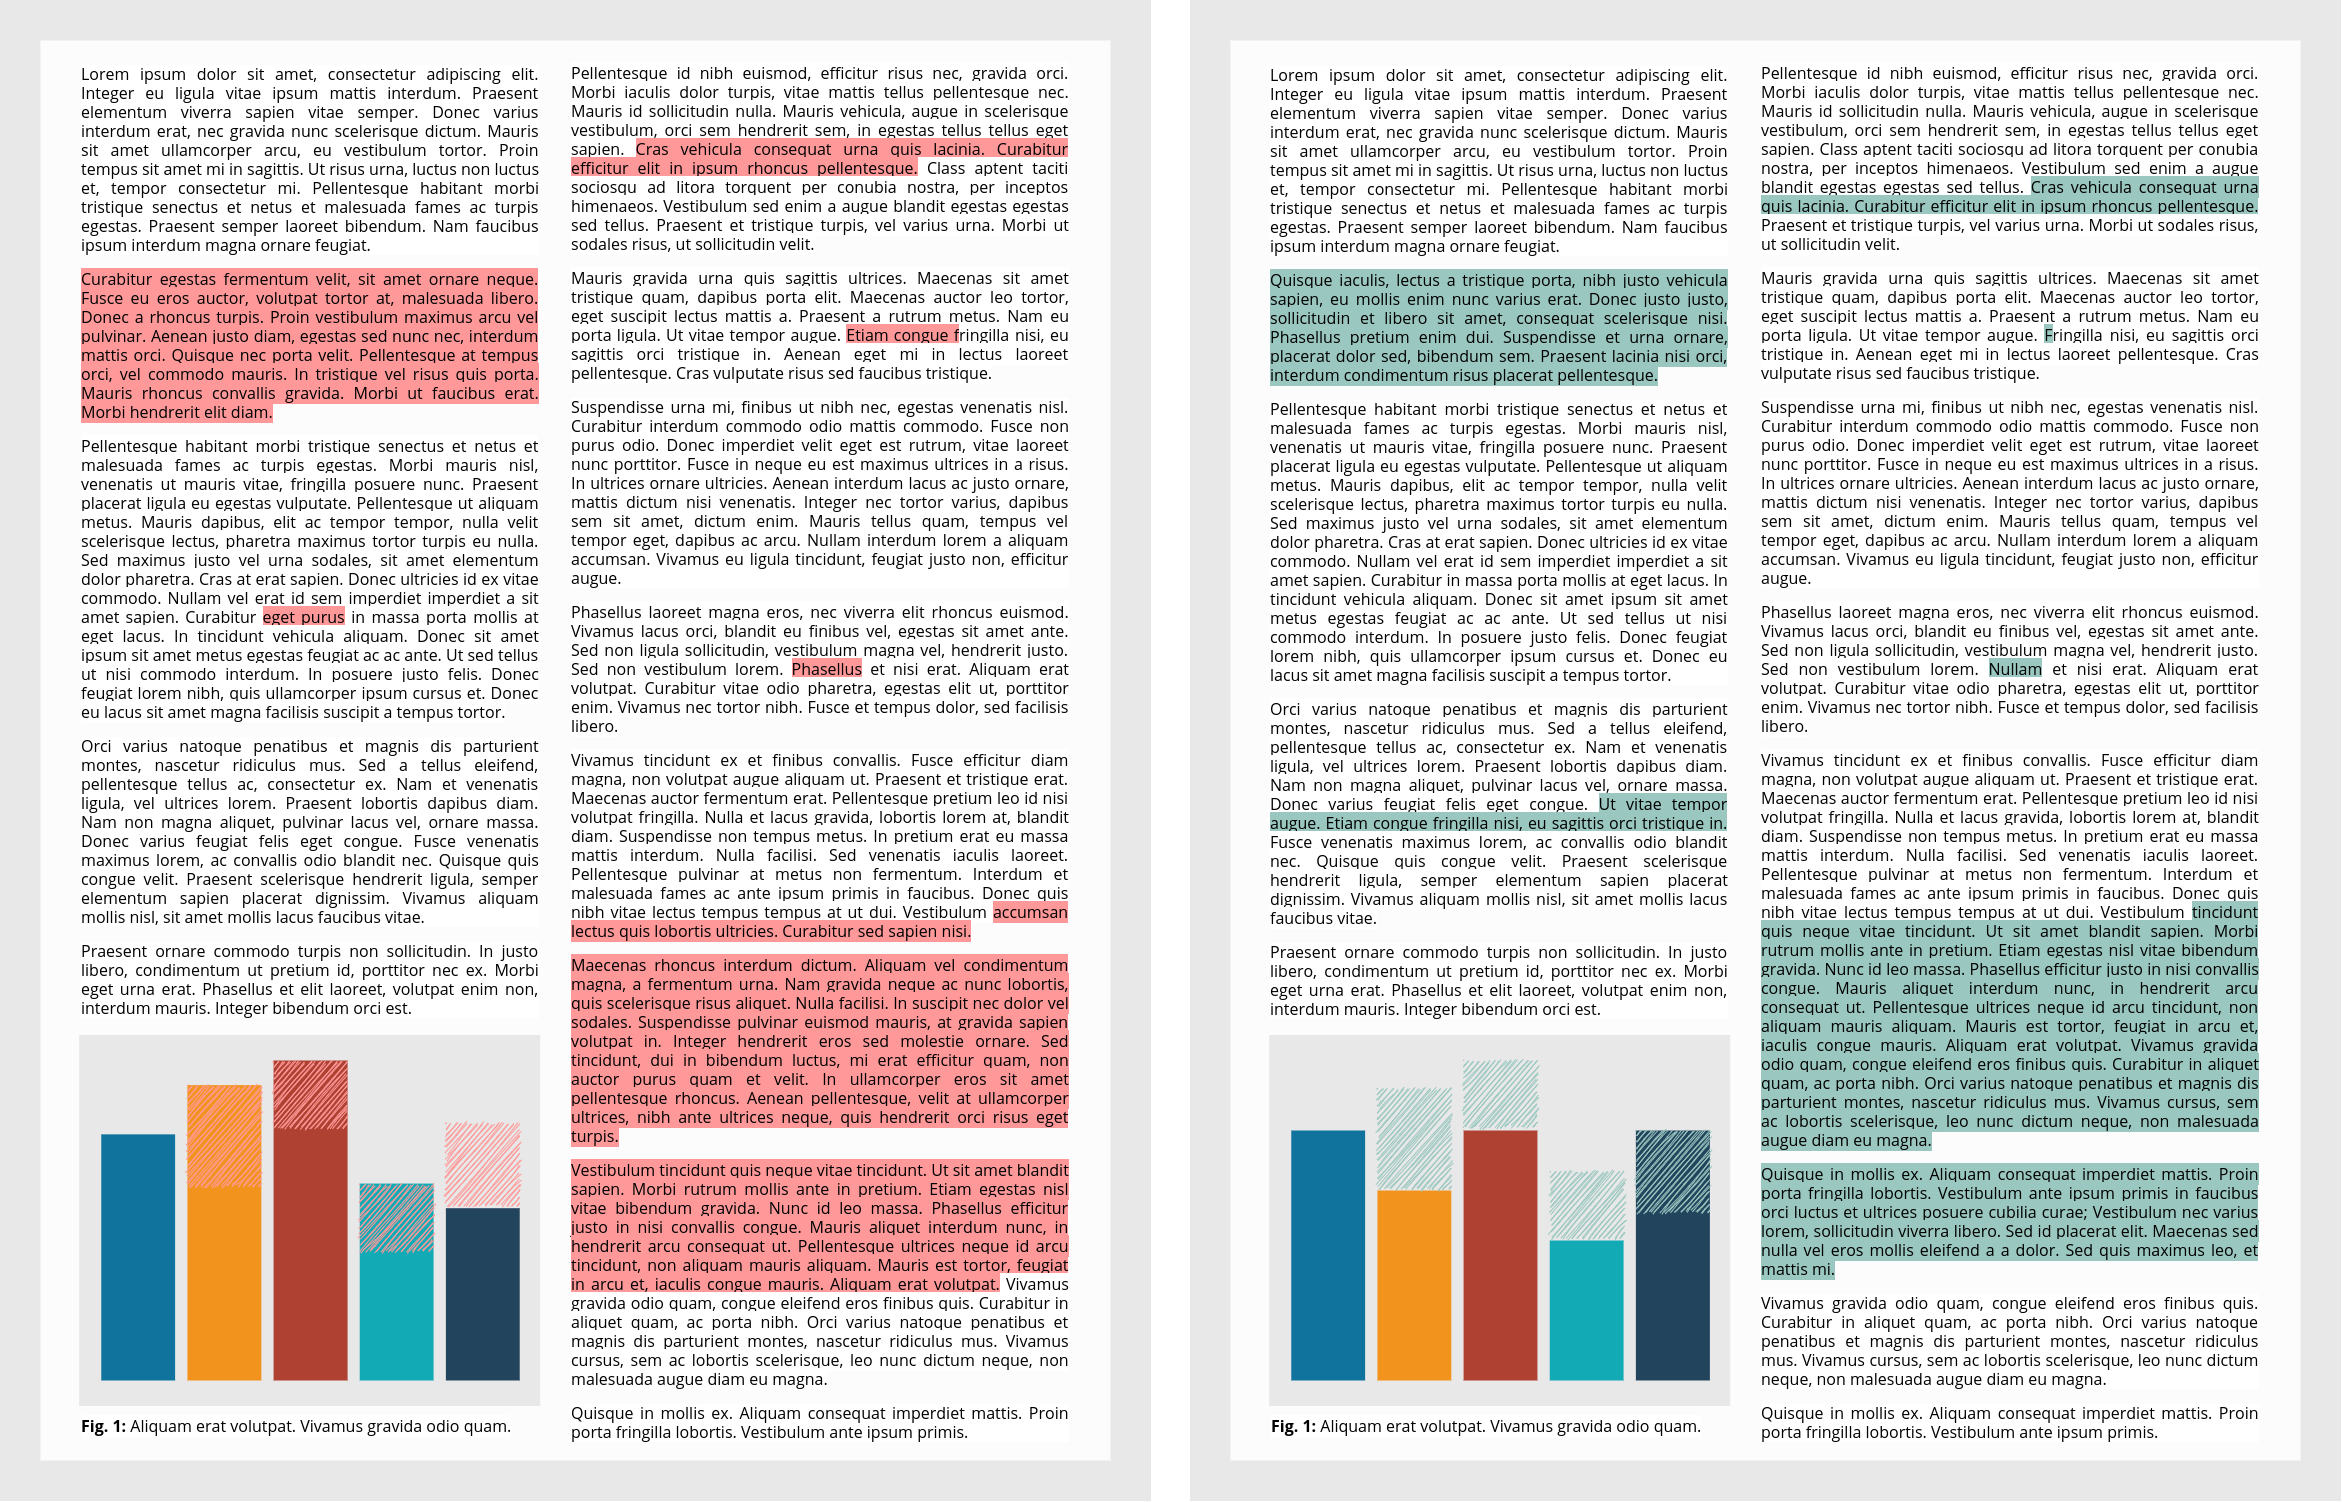
\includegraphics[width=0.48\textwidth]{figures/paper-pdf-delta.png}
    \caption{Detailed visual comparison report (mock-up); left shows what has been removed in the previous version's PDF, right shows what has been added to the latest version's PDF.}
    \label{fig:paper-pdf-delta}
\end{figure}

%%%%%%%%%%%%%%%%%%%%%%%%%%%%%%%%%%%%%%%%%%%%
%%%%%%%%%%%%%%%%%%%%%%%%%%%%%%%%%%%%%%%%%%%%
%%%%%%%%%%%%%%%%%%%%%%%%%%%%%%%%%%%%%%%%%%%%
%%%%%%%%%%%%%%%%%%%%%%%%%%%%%%%%%%%%%%%%%%%%
%%%%%%%%%%%%%%%%%%%%%%%%%%%%%%%%%%%%%%%%%%%%

\clearpage

\begin{table*}[b]
    \centering
    \caption{NSDI '20 analysis overview ordered by program appearance.}\vspace{3pt}
    \begin{tabular}{| C{0.55cm} | C{0.65cm} || C{0.9cm} | C{0.8cm} | C{0.95cm} | C{1.1cm} | C{0.5cm} | } \hline
        \textbf{\#} & \textbf{Ref.} & \textbf{Tweak} & \textbf{C/S/E} & \textbf{Cloud} & \textbf{Custom} & \textbf{DS} \\ \hline
%%%%%%%%%%%%%%%%%%%%%%%%%%%%%%
1 & \cite{nsdi-2020-mellette} & \checkmark & \checkmark &  & \checkmark &  \\ \hline
2 & \cite{nsdi-2020-cheng} & \checkmark & \checkmark &  & \checkmark &  \\ \hline
3 & \cite{nsdi-2020-jha} &  &  &  & \checkmark & \checkmark \\ \hline
4 & \cite{nsdi-2020-alcoz} & \checkmark & \checkmark &  & \checkmark &  \\ \hline
5 & \cite{nsdi-2020-moon} & \checkmark &  &  & \checkmark &  \\ \hline
6 & \cite{nsdi-2020-arashloo} & \checkmark & \checkmark &  & \checkmark &  \\ \hline
7 & \cite{nsdi-2020-yang} & \checkmark &  &  & \checkmark &  \\ \hline
8 & \cite{nsdi-2020-hwang} & \checkmark &  &  & \checkmark &  \\ \hline
9 & \cite{nsdi-2020-kuga} & \checkmark &  &  & \checkmark &  \\ \hline
10 & \cite{nsdi-2020-uluyol} & \checkmark &  & \checkmark &  &  \\ \hline
11 & \cite{nsdi-2020-yuan} &  & \checkmark & \checkmark &  &  \\ \hline
12 & \cite{nsdi-2020-abhashkumar} &  & \checkmark &  &  &  \\ \hline
13 & \cite{nsdi-2020-zhang-kaiyuan} &  & \checkmark &  & \checkmark &  \\ \hline
14 & \cite{nsdi-2020-zhang-peng} &  & \checkmark &  &  &  \\ \hline
15 & \cite{nsdi-2020-yousefi} &  & \checkmark &  &  &  \\ \hline
16 & \cite{nsdi-2020-lai} & \checkmark &  & \checkmark &  &  \\ \hline
17 & \cite{nsdi-2020-mahajan} & \checkmark & \checkmark & \checkmark &  &  \\ \hline
18 & \cite{nsdi-2020-liu-ming} & \checkmark &  &  & \checkmark &  \\ \hline
19 & \cite{nsdi-2020-ding} & \checkmark & \checkmark & \checkmark &  &  \\ \hline
20 & \cite{nsdi-2020-gadre} &  &  &  & \checkmark &  \\ \hline
21 & \cite{nsdi-2020-goyal} & \checkmark & \checkmark &  & \checkmark &  \\ \hline
22 & \cite{nsdi-2020-carver} &  &  &  & \checkmark &  \\ \hline
23 & \cite{nsdi-2020-li} & \checkmark &  &  & \checkmark &  \\ \hline
24 & \cite{nsdi-2020-mogul} &  &  &  &  &  \\ \hline
25 & \cite{nsdi-2020-agache} & \checkmark &  & \checkmark &  &  \\ \hline
26 & \cite{nsdi-2020-mehta} &  &  &  & \checkmark &  \\ \hline
27 & \cite{nsdi-2020-vuppalapati} &  &  &  & \checkmark & \checkmark \\ \hline
28 & \cite{nsdi-2020-brooker} & \checkmark & \checkmark &  & \checkmark &  \\ \hline
29 & \cite{nsdi-2020-vermeulen} &  &  & \checkmark &  & \checkmark \\ \hline
30 & \cite{nsdi-2020-yan} & \checkmark &  & \checkmark & \checkmark &  \\ \hline
31 & \cite{nsdi-2020-uta} & \checkmark &  & \checkmark &  &  \\ \hline
32 & \cite{nsdi-2020-song} & \checkmark & \checkmark & \checkmark &  &  \\ \hline
33 & \cite{nsdi-2020-hauer} &  &  &  & \checkmark &  \\ \hline
34 & \cite{nsdi-2020-lou} & \checkmark &  & \checkmark &  &  \\ \hline
%%%%%%%%%%%%%%%%%%%%%%%%%%%%%%
    \end{tabular}
    \hspace{0.2cm}
    \begin{tabular}{| C{0.55cm} | C{0.65cm} || C{0.9cm} | C{0.8cm} | C{0.95cm} | C{1.1cm} | C{0.5cm} | } \hline
        \textbf{\#} & \textbf{Ref.} & \textbf{Tweak} & \textbf{C/S/E} & \textbf{Cloud} & \textbf{Custom} & \textbf{DS} \\ \hline
%%%%%%%%%%%%%%%%%%%%%%%%%%%%%%
35 & \cite{nsdi-2020-zhai} & \checkmark &  &  & \checkmark &  \\ \hline
36 & \cite{nsdi-2020-burke} & \checkmark &  & \checkmark &  &  \\ \hline
37 & \cite{nsdi-2020-hu-jiyao} & \checkmark & \checkmark &  &  & \checkmark \\ \hline
38 & \cite{nsdi-2020-levai} & \checkmark &  &  & \checkmark &  \\ \hline
39 & \cite{nsdi-2020-mukerjee} & \checkmark &  & \checkmark & \checkmark &  \\ \hline
40 & \cite{nsdi-2020-barbette} & \checkmark &  &  & \checkmark &  \\ \hline
41 & \cite{nsdi-2020-sharma} & \checkmark & \checkmark &  & \checkmark &  \\ \hline
42 & \cite{nsdi-2020-hsu} & \checkmark & \checkmark & \checkmark &  &  \\ \hline
43 & \cite{nsdi-2020-takruri} & \checkmark &  &  & \checkmark &  \\ \hline
44 & \cite{nsdi-2020-pouryousef} & \checkmark &  & \checkmark &  &  \\ \hline
45 & \cite{nsdi-2020-kwon} & \checkmark &  & \checkmark &  &  \\ \hline
46 & \cite{nsdi-2020-sivaraman} & \checkmark & \checkmark &  &  &  \\ \hline
47 & \cite{nsdi-2020-arzani} & \checkmark &  &  & \checkmark & \checkmark \\ \hline
48 & \cite{nsdi-2020-hunt} & \checkmark & \checkmark & \checkmark &  &  \\ \hline
49 & \cite{nsdi-2020-burkhalter} & \checkmark &  & \checkmark & \checkmark &  \\ \hline
50 & \cite{nsdi-2020-hu-yuncong} & \checkmark &  & \checkmark &  &  \\ \hline
51 & \cite{nsdi-2020-mardani} &  &  &  & \checkmark &  \\ \hline
52 & \cite{nsdi-2020-liu-xin} &  &  &  & \checkmark &  \\ \hline
53 & \cite{nsdi-2020-kumar} &  &  &  & \checkmark &  \\ \hline
54 & \cite{nsdi-2020-zhao} &  &  &  & \checkmark &  \\ \hline
55 & \cite{nsdi-2020-prabhu} &  & \checkmark &  &  &  \\ \hline
56 & \cite{nsdi-2020-birkner} &  & \checkmark &  &  &  \\ \hline
57 & \cite{nsdi-2020-burnett} &  &  &  & \checkmark &  \\ \hline
58 & \cite{nsdi-2020-kakarla} &  & \checkmark &  &  &  \\ \hline
59 & \cite{nsdi-2020-yaseen} & \checkmark &  &  & \checkmark &  \\ \hline
60 & \cite{nsdi-2020-hessar} &  &  &  & \checkmark &  \\ \hline
61 & \cite{nsdi-2020-arun} &  &  &  & \checkmark &  \\ \hline
62 & \cite{nsdi-2020-ahmad} &  & \checkmark &  & \checkmark &  \\ \hline
63 & \cite{nsdi-2020-ha} &  &  &  & \checkmark &  \\ \hline
64 & \cite{nsdi-2020-chen} &  &  &  & \checkmark &  \\ \hline
65 & \cite{nsdi-2020-ayyalasomayajula} &  &  &  & \checkmark &  \\ \hline
%%%%%%%%%%%%%%%%%%%%%%%%%%%%%%
 &  &  &  &  &  & \\ \hline
 \multicolumn{2}{| c ||}{\textbf{Total}} & \textbf{38} & \textbf{23} & \textbf{19} & \textbf{40} & \textbf{5} \\ \hline
 \multicolumn{2}{| c ||}{\textbf{Fraction}} & \textbf{58\%} & \textbf{35\%} & \textbf{29\%} & \textbf{62\%} & \textbf{8\%} \\ \hline
    \end{tabular}
\label{tab:nsdi2020}
\end{table*}

\section{NSDI 2020 analysis}
\label{appendix:nsdianalysis}

In order to assess the applicability of \sysname, we went through the 65 papers of NSDI 2020. For each paper we registered the following characteristics:

\begin{itemize}[leftmargin=10pt,itemsep=2pt,topsep=2pt]

    \item \textbf{Tweak:} Whether we could identify experimental setup parameters which could be of interest for the reader to tweak with \sysname. Certain types of work are \textbf{excluded} even though they may have parameters or configurations of interest:
    
    \begin{itemize}[leftmargin=10pt,itemsep=2pt,topsep=2pt]
        \item Predominantly measurement studies
        \item Custom hardware wireless communication systems in the physical world (as setup involves physical steps)
        \item Verification systems (as the outcome is typically binary)
        \item Operational experience studies
    \end{itemize}

    \item \textbf{C/S/E:} The presence of experiments aimed to be run over general compute: \textbf{C}alculation, \textbf{S}imulation or \textbf{E}mulation. This excludes emulated deployments of the system on external cloud infrastructure as they fall into the next category.
    
    \item \textbf{Cloud:} The presence of explicit system deployment experiments using publicly accessible (cloud) infrastructure (\eg PlanetLab, Emulab, AWS, Azure, Google Cloud).
    
    \item \textbf{Custom:} The presence of experiments using custom hardware (\eg custom chips) or non-public infrastructure.
    
    \item \textbf{Dataset (DS):} The paper explicitly showcases a dataset. (We do not check for public availability of the dataset.)
    
\end{itemize}

\noindent When in doubt, \eg for research problems we have less familiarity with, we leaned towards a conservative analysis, \eg not checking the box for interesting parameters to tweak, if we were unsure. The results are displayed in Table~\ref{tab:nsdi2020}.

%%%%%%%%%%%%%%%%%%%%%%%%%%%%%%%%%%%%%%%%%%%%
%%%%%%%%%%%%%%%%%%%%%%%%%%%%%%%%%%%%%%%%%%%%
%%%%%%%%%%%%%%%%%%%%%%%%%%%%%%%%%%%%%%%%%%%%
%%%%%%%%%%%%%%%%%%%%%%%%%%%%%%%%%%%%%%%%%%%%
%%%%%%%%%%%%%%%%%%%%%%%%%%%%%%%%%%%%%%%%%%%%

\clearpage
\section{Replication instructions}

Below we detail the replication instructions. It assumes Ubuntu LTE 18.04, 20.04 or later, and Python version 3.7 or higher (with \texttt{pip} installed). Additional information can be found in the \texttt{README.md} of the code repository.

\begin{enumerate}
    \item Clone (or download from the venue website) the code repository and navigate into it:\\
    \\
    \texttt{git clone https://github.com/snkas/codebind-paper.git}\\
    \texttt{cd codebind-paper}\\

    \item Setup environment (\ie install dependencies) (duration: $\pm$8~min.):\\
    \\
    \texttt{bash setup\_env.sh}\\

    \item (\textit{Optional}) It takes quite some time for the next step (reproduce) to rerun all experiments, as such for convenience an archive with the runs already finished is provided:\\
    \\
    \texttt{mkdir -p temp}\\
    \texttt{tar -xzf partial-temp-runs.tar.gz -C temp}\\
    \\
    Skip this step if you wish to replicate from scratch.\\

    \item Reproduce the paper (duration: $\pm$8~hours without optional extraction, $\pm$15-20~min. with):\\
    \\
    \texttt{bash reproduce.sh}\\

    \item The paper is output at: \texttt{paper-latex/out/paper.pdf}\\

\end{enumerate}

\noindent We also provide a short (5:31) video demonstration of the process (please set quality manually to 720p):\\

\noindent\url{https://drive.google.com/file/d/1f8gu3MpWzXM4WbpFLy7DXDcR4z3s6Ws9/view}\\

\noindent \textit{The code repository makes use of ns-3~\cite{ns3}, the basic-sim ns-3 module \cite{basic-sim}, top-lists~\cite{top-lists}, ACM LaTeX class files~\cite{acm-latex}, and several gnuplot files. See the complete license at ./LICENSE for more detailed information. It moreover makes use of several distribution packages (texlive~\cite{texlive}, gnuplot~\cite{gnuplot}, openmpi~\cite{openmpi}, lcov~\cite{lcov}) and Python modules (texsoup~\cite{texsoup}, exputilpy~\cite{exputilpy}, networkx~\cite{networkx}, matplotlib~\cite{matplotlib}, pandas~\cite{pandas}, numpy~\cite{numpy}, statsmodels~\cite{statsmodels}).}


\end{document}
